\chapter{相关研究基础}
自从计算机技术应用到医学影像分析以来,有许许多多医学影像分析难题因其具有的重大临床应用价值和实际意义而引起研究者的浓厚兴趣并为之投入大量时间和精力,疾病标记物的精确定位便是其中之一。本章将会介绍本文后续内容涉及到的基本知识点。接着,我们将会介绍与疾病标记物定位任务相关的研究进展,力求将相关方法阐述得清晰明了,突出比较各种方法在疾病标记物定位任务上的长处和不足。在本章最后,我们将给出实验结果的评判标准并介绍与疾病标记物定位任务相关的数据集。

\section{相关基础}
%本小节主要是介绍疾病标记物定位任务的概念和目前常用的模型方法。我们首先会介绍CNN、编码器-解码器等重要基本要点。接着介绍目前已有的常用解决模型方法。最后介绍对各种模型方法性能比较的评价标准。

%\subsection{疾病标记物定位任务}\label{subsec:bio_loc_task_definition}
%\begin{figure}[h]
%	\centering
%	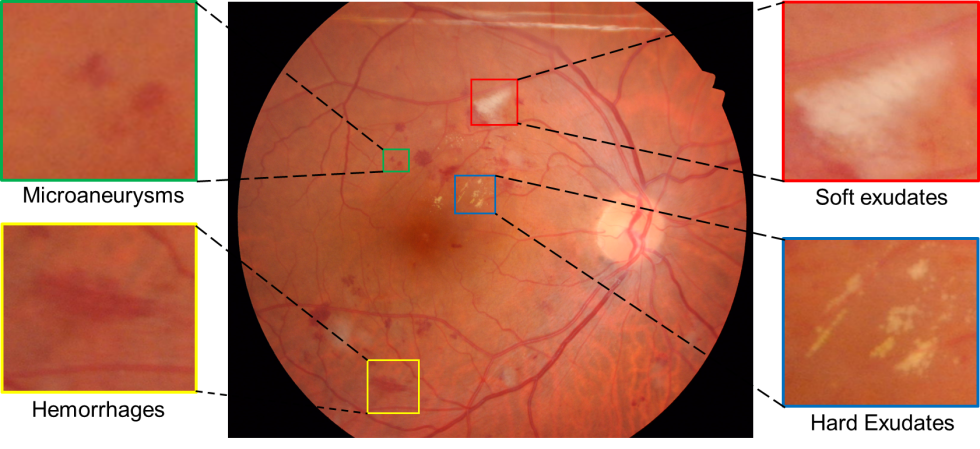
\includegraphics[width=1.0\textwidth]{figure/biomarker_localization_example}
%	\caption{疾病标记物定位任务示例。红色矩形框、绿色矩形框、蓝色矩形框和黄色矩形框标记了四种糖尿病视网膜病变的异常表现,分别代表软性渗出液(Soft Exudates)、微动脉瘤
%		(Microaneurysms)、硬性渗出液(Hard Exudates)和出血(Hemorrhages)。} 
%	\label{fig:biomarker_localization_example}
%\end{figure}
%生物标志物是开发新疗法和辅助诊断的关键,受到研究人员的不断关注,其目标是为合适的病人开发合适的药物。随着计算机视觉技术不断应用到医学领域,疾病标记物定位任务自然也变成了研究热点。在医学影像处理领域,一旦一张医学影像被诊断为某种特定疾病,疾病标记物定位任务的目标便是寻找其患病区域,或者说在图像上找到诊断依据,该依据或者患病区域即可看作是疾病标记物。如图\ref{fig:biomarker_localization_example},该图像被诊断为患有糖尿病视网膜病变,疾病标记物定位任务便是找到其异常表现,并给出其准确位置。可以发现,糖尿病视网膜病变有多种异常表现,疾病标记物定位任务要求不能漏检。另外,可以发现从颜色特征上看,出血(图中黄色矩形框)异常和眼底血管非常相似,因而将微小血管看作异常表现的假阳现象也可能发现。以上均给疾病标记物定位任务增加了不少难度。如果将CNN手段,根据以上介绍,疾病标记物定位任务的目标是找出疾病诊断背后的诊断依据,这与CNN的可视化/可解释性的目标恰好一致,因此CNN的可视化/可解释性是疾病标记物定位任务的主要解决方案之一。相关内容将会在\ref{subsec:visulization_methods}小节详细叙述。
\subsection{卷积神经网络}\label{subsec:cnn_introduction}
CNN最初是为了避免传统神经网络(多层感知机)在处理图像时的缺点而提出的。多层感知机在处理图像数据时,多层感知机对每张输入图像中的每个像素点都使用一个感知器。对于较大的图像,权重的数量很快就变得难以管理。例如,对于一个有3个彩色通道的224$\times$224像素图像,大约需要训练150,000个参数。此时,巨大参数量导致多层感知机的训练变得十分困难。另外,多层感知机不具备平移不变性。例如,如果一张猫出现在一张图像的左上角和另一张图像的右下角,多层感知机将假设猫总是出现在图片的这个位置。多层感知机在处理图像时还需要将二维图像数据转为一维向量形式存在,这导致多层感知机无法利用二维空间的相对位置信息。

\begin{figure}[h!] % image examples & compare
	\centering
	\begin{subfigure}{0.35\textwidth}
		\centering
		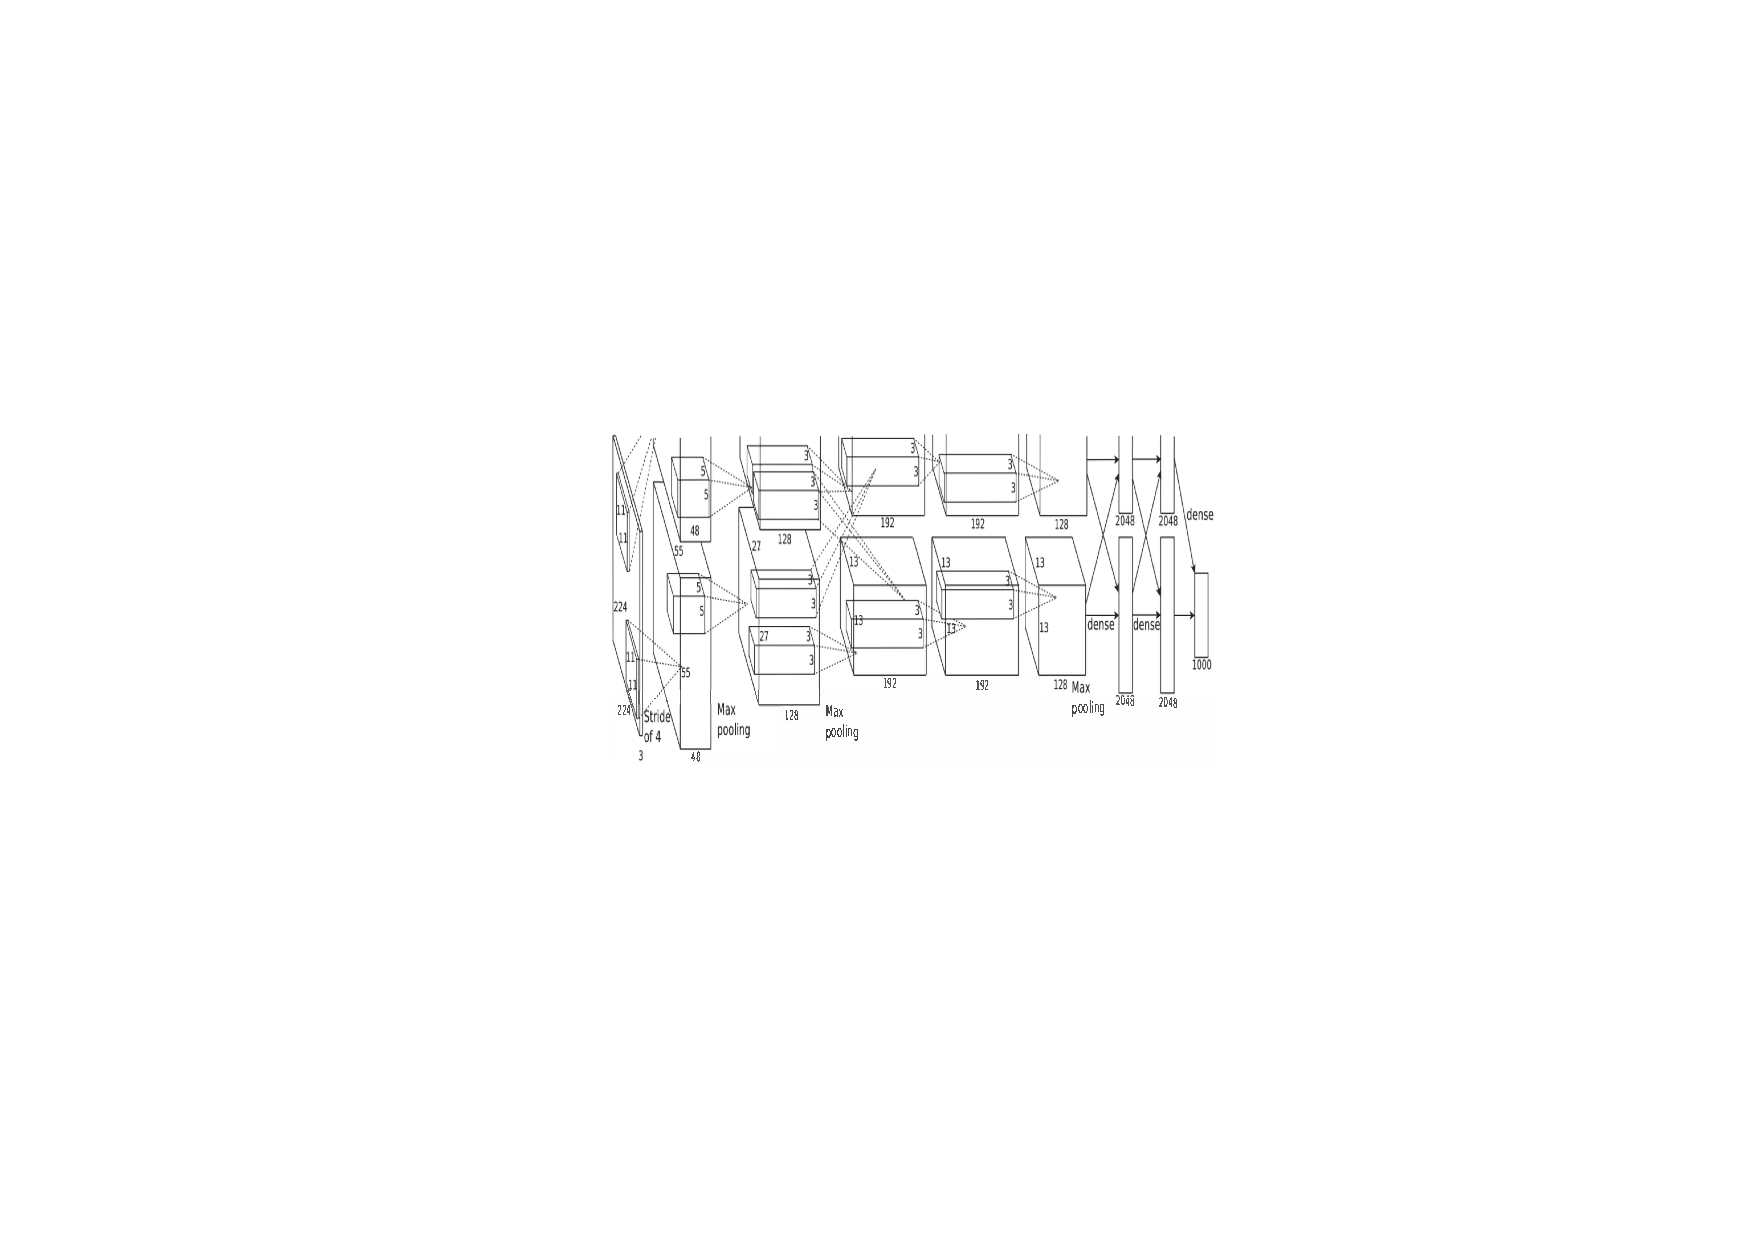
\includegraphics[width=1.0\textwidth]{figure/popular_networks_alex_net}
		\caption{AlexNet~\cite{krizhevsky2012imagenet}}
		\label{subfig1}
	\end{subfigure}
	\quad
	\begin{subfigure}{0.336\textwidth}
		\centering
		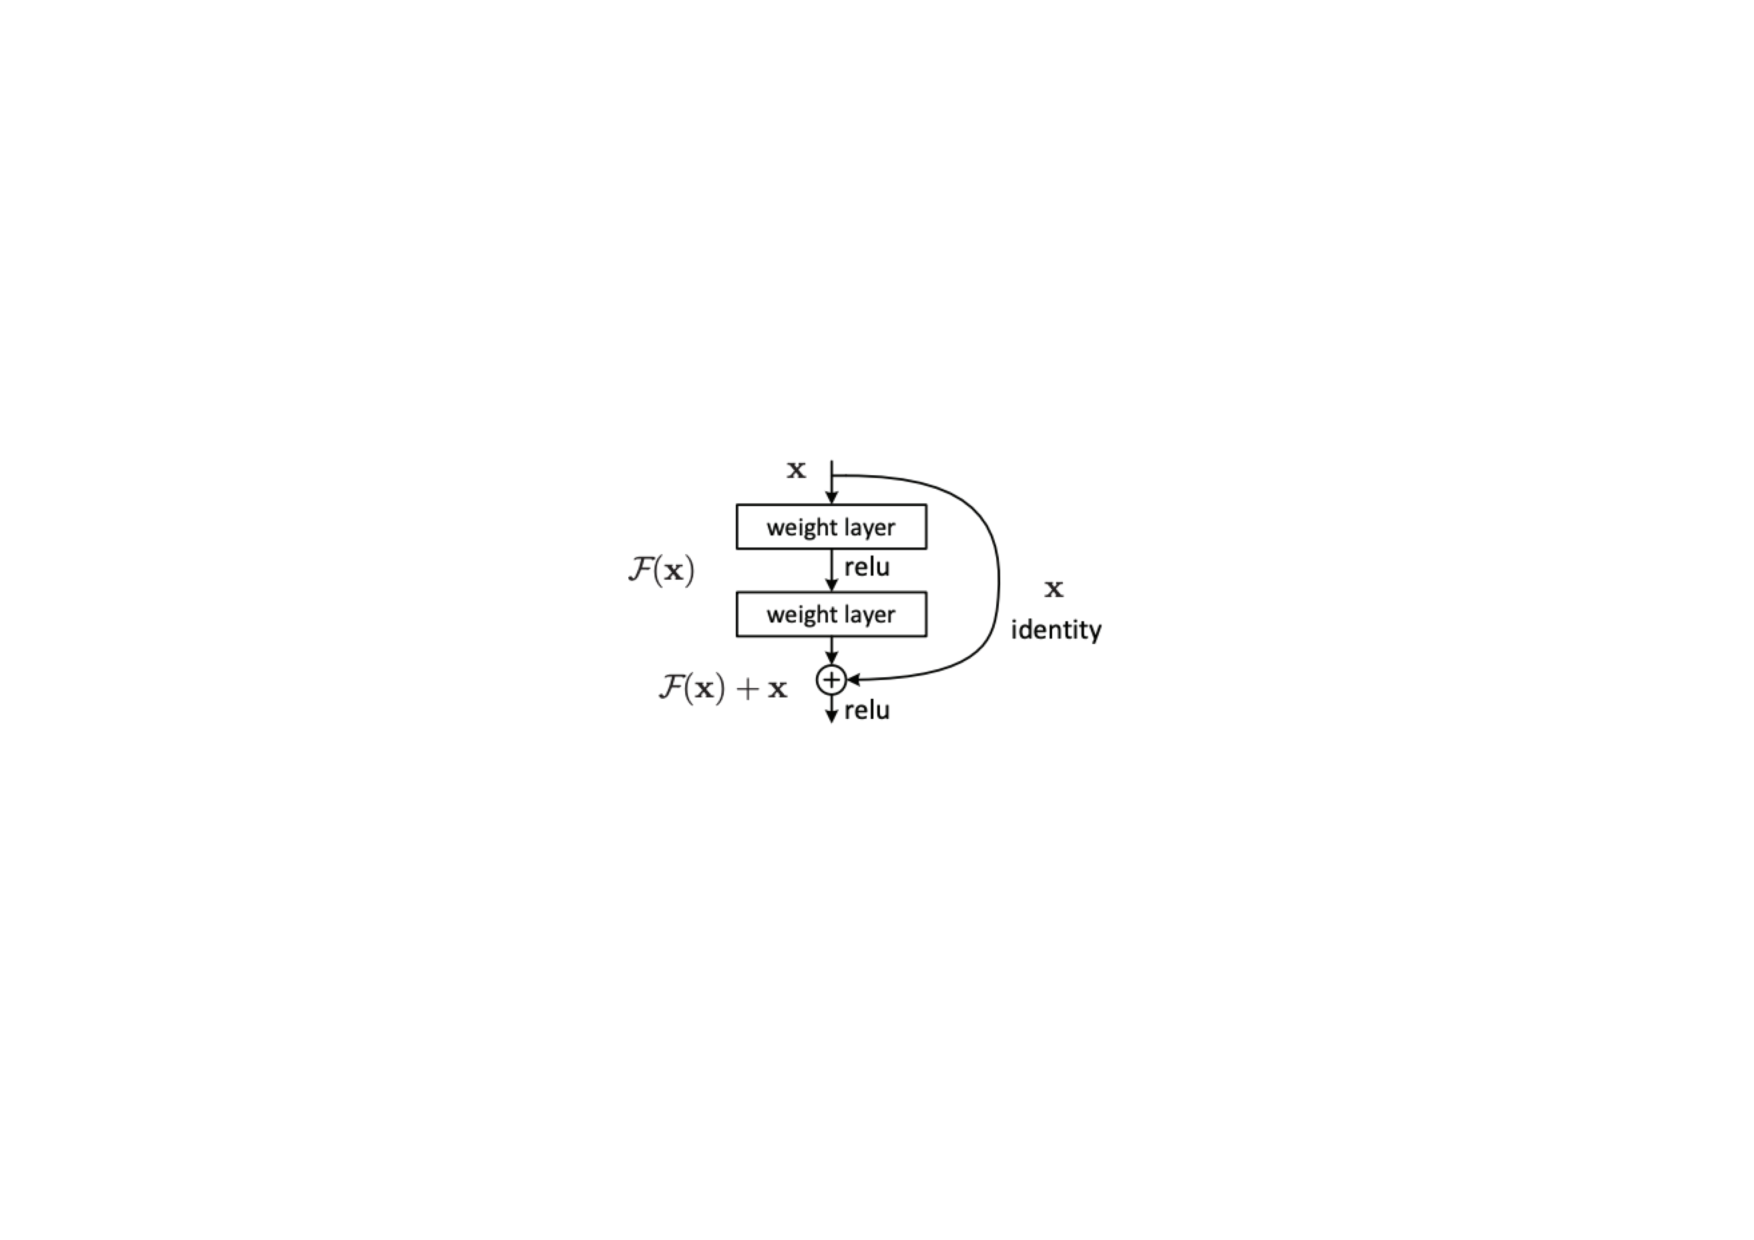
\includegraphics[width=1.0\textwidth]{figure/popular_networks_resnet}
		\caption{ResNet残差单元~\cite{he2016deep}}
		\label{subfig:resnet_block}
	\end{subfigure}
	\begin{subfigure}{0.265\textwidth}
		\centering
		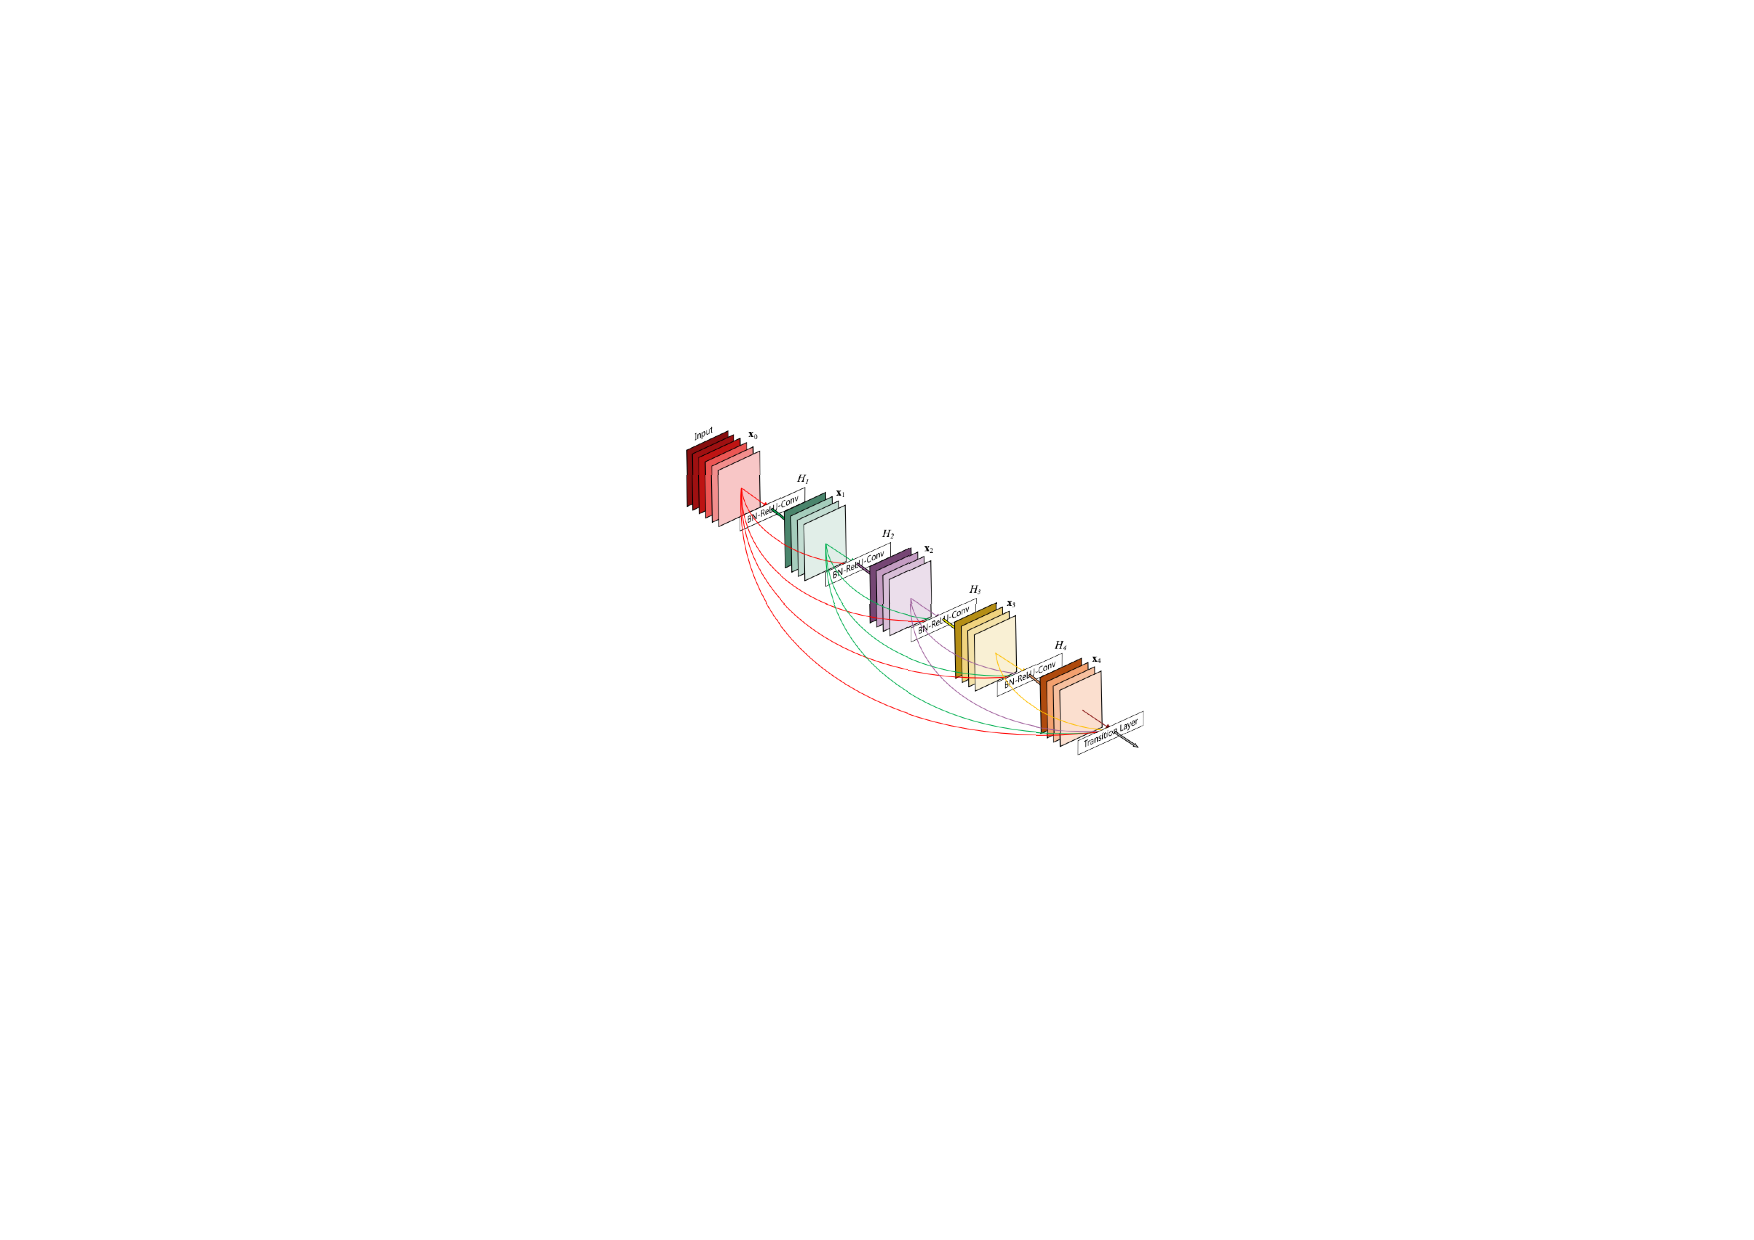
\includegraphics[width=1.0\textwidth]{figure/popular_networks_densenet}
		\caption{DenseNet~\cite{huang2017densely}}
	\end{subfigure}
	\caption[三种经典CNN模型]{三种经典CNN模型(图片均来自于对应论文~\cite{krizhevsky2012imagenet, he2016deep, huang2017densely})。子图\ref{subfig:resnet_block}为残差单元,ResNet网络实际上由多个残差单元堆叠组成。} 
	\label{mulfig:popular_networks}
\end{figure}

%CNN便可以很好避免多层感知机存在的问题,卷积操作可以很好的捕捉图像的空间信息。另外,卷积操作还具有平移不变性。权值共享机制可以大大降低参数量。随着计算机算力的快速提升,运用反向传播算法~\cite{hecht1992theory},CNN的大规模训练变得切实可行。自Hinton等人利用两块GPU成功训练AlexNet~\cite{krizhevsky2012imagenet}后,很多优秀网络结构被提出,比如VGG~\cite{simonyan2014very},ResNet~\cite{he2016deep, he2016identity},DenseNet~\cite{huang2017densely},Inception系列网络~\cite{szegedy2015going, szegedy2016rethinking, szegedy2017inception}。CNN除了在分类问题上取得出色性能外,还在自然语言处理~\cite{dos2014deep, mou2016convolutional, li2019knowledge}、无人驾驶~\cite{lee2017deep, csillik2018identification, tang2017vehicle}、语音识别~\cite{abdel2013exploring, swietojanski2014convolutional, robertson2019exploring}等领域表现不凡,越来越受到研究者们的青睐。

CNN可以很好避免多层感知机存在的问题,首先用CNN处理图像时直接用矩阵来表示图像数据,无须将其转化为一维向量,因此卷积操作可以很好地捕捉图像的空间信息和上下文信息。除此之外,卷积操作还具有平移不变性,CNN中权值共享机制可以大大降低参数量。随着图形处理器(Graphics Processing Unit,缩写为GPU)的广泛应用和快速迭代,计算机的算力也快速提升,运用反向传播算法~\cite{hecht1992theory},CNN的大规模部署与训练变得切实可行。因此,自从Hinton等人~\cite{krizhevsky2012imagenet}利用两块GPU成功训练AlexNet后,很多优秀网络结构相继被提出,比如,VGG~\cite{simonyan2014very},ResNet~\cite{he2016deep, he2016identity}和DenseNet~\cite{huang2017densely}。CNN除了在分类问题上表现出出色性能外,还在自然语言处理~\cite{dos2014deep, mou2016Convolutional}、无人驾驶~\cite{lee2017deep}等领域表现不凡,越来越受到研究者们的青睐。

三种经典的CNN的模型结构如图~\ref{mulfig:popular_networks}所示。图中从左到右,三种网络结构依次为AlexNet~\cite{krizhevsky2012imagenet}、ResNet残差单元(ResNet实际上是由多个残差单元堆叠组成)~\cite{he2016deep, he2016identity}和DenseNet~\cite{huang2017densely}。可以看出,CNN都是由一系列卷积操作组成的,在卷积操作之后再接上激活函数以增强非线性表达能力。为了减少参数量,CNN除了引入权值共享机制外,还引入了池化操作,使得输入图像尺寸随着深度不断增加而减小,与此同时池化操作还起到过滤无关信息的的作用。为了增强CNN的非线性表达能力,可在CNN中添加激活函数。最后,再接上全连接层对提取到的特征进行分类(视不同任务而改变)。在此过程中,CNN实际上充当特征提取器的角色。那么我们可以这样理解CNN:CNN是一种层次化结构,单纯卷积操作提取的是图像的局部信息,随着一系列卷积操作的堆叠,CNN的感受野越来越大,比如两个3$\times$3的卷积核堆叠相当于一个5$\times$5卷积核的感受野,CNN便能提取到图像的全局信息。激活函数可增强CNN的非线性表达能力。随着深度增加,为了减少参数量,可添加池化层使输入卷积层的尺寸变小。采用这种层次化结构,CNN可逐步提取到输入图像与特定任务相关的高层语义特征。在损失函数(比如交叉熵)的监督指导下,运用梯度反向传播算法计算梯度更新网络参数,CNN便能被训练成一个良好的特征提取器。

%以上便是CNN的一般结构和工作原理,由于ResNet-18在本文提出的方法充当重要角色,下面将详细介绍ResNet模型。随着VGG-19~\cite{simonyan2014very}的出现,一个CNN的深度越深,学出来的效果是否越好的问题摆在了研究者们的面前。由于CNN的深度越深,原本就存在的过拟合和梯度消失问题变得越严重。何凯明等人便设计了一种在深度远大于VGG-19,效果也由于VGG-19的网络模型。设$\mathcal{H}(x)$是CNN拟合的函数,$x$表示网络输入。如果假设多个非线性层可以渐近逼近复杂函数并且假设输入和输出尺寸相同,那么就可以假设它们可以渐近逼近残差函数$\mathcal{F}(x)$,即$\mathcal{F}(x)=\mathcal{H}(x)− x$。因此,ResNet没有让网络直接拟合$\mathcal{H}(x)$,而是明确地让这些层近似为残差函数$\mathcal{F}(x)=\mathcal{H}(x)-x$。 因此,原始函数变为$\mathcal{F}(x)+x$。尽管两种形式都应能够渐近地逼近所需的功能(如假设),但是近似拟合残差函数要容易得多。另外,为了表示加号,残差单元中通常加入跳接操作。

%设$\boldsymbol{X}_l$表示第$l$个残差单元的输入,$\boldsymbol{W}_{l}=\{\boldsymbol{W}_{l,k}|_{1\leq k \leq K}\}$表示第$l$个残差单元的权重,$K$表示残差单元个数。则相邻的残差单元输入$\boldsymbol{X}_{l+1}$可以表示为:
%\begin{gather*}
%	\boldsymbol{Y}_{l}=\boldsymbol{X}_l + \mathcal{F}(\boldsymbol{X}_l, \boldsymbol{W}_l), \\
%	\boldsymbol{X}_{l+1}=f(\boldsymbol{Y}_{l}).
%\end{gather*}
%其中$f$表示激活函数,$\mathcal{F}(\boldsymbol{X}_l, \boldsymbol{W}_l)$表示残差单元中的卷积操作。如果$f$表示恒等变换,则$\boldsymbol{X}_{l+1}=\boldsymbol{Y}_{l}$,有:
%\begin{equation*}
%	\boldsymbol{X}_{l+1}=\boldsymbol{X}_l + \mathcal{F}(\boldsymbol{X}_l, \boldsymbol{W}_l).
%\end{equation*}
%对于任意第$L(L\ge l)$个残差单元,其输入$\boldsymbol{X}_{L}$,可写为:
%\begin{equation}\label{equ:residual_block_compute}
%\boldsymbol{X}_{L}=\boldsymbol{X}_l + \sum_{i=l}^{L-1}\mathcal{F}(\boldsymbol{X}_i, \boldsymbol{W}_i).
%\end{equation}
%设损失函数为$\boldsymbol{\varepsilon}$,根据等式\ref{equ:residual_block_compute}和反向梯度传播算法的链式求导法有:
%\begin{equation}\label{residual_block_gradient}
%\frac{\partial \boldsymbol{\varepsilon}}{\partial \boldsymbol{X}_l}=\frac{\partial \boldsymbol{\varepsilon}}{\partial \boldsymbol{X}_L}\frac{\partial \boldsymbol{X}_L}{\partial \boldsymbol{X}_l}=\frac{\partial \boldsymbol{\varepsilon}}{\partial \boldsymbol{X}_L}(1+\frac{\partial}{\partial \boldsymbol{X}_l}\sum_{i=l}^{L-1}\mathcal{F}(\boldsymbol{X}_i,\boldsymbol{W}_i)).
%\end{equation}
%等式\ref{residual_block_gradient}表明,梯度$\frac{\partial \boldsymbol{\varepsilon}}{\partial \boldsymbol{X}_l}$由$\frac{\partial \boldsymbol{\varepsilon}}{\partial \boldsymbol{X}_L}$和$\frac{\partial \boldsymbol{\varepsilon}}{\partial \boldsymbol{X}_L}\frac{\partial}{\partial \boldsymbol{X}_l}\sum_{i=l}^{L-1}\mathcal{F}(\boldsymbol{X}_i,\boldsymbol{W}_i)$两项组成。第一项在可直接传播信息而与任意残差单元无关。而第二项保证信息直接回传到上一个残差单元。由于第一项的存在,等式\ref{residual_block_gradient}还能保证每一层梯度不容易消失,即使在残差单元权重很小的情况下。ResNet具有优异性能,深度达到上千层仍不会发生梯度消失现象。

\subsection{编码器-解码器}

%\begin{figure}[h]
%	\centering
%	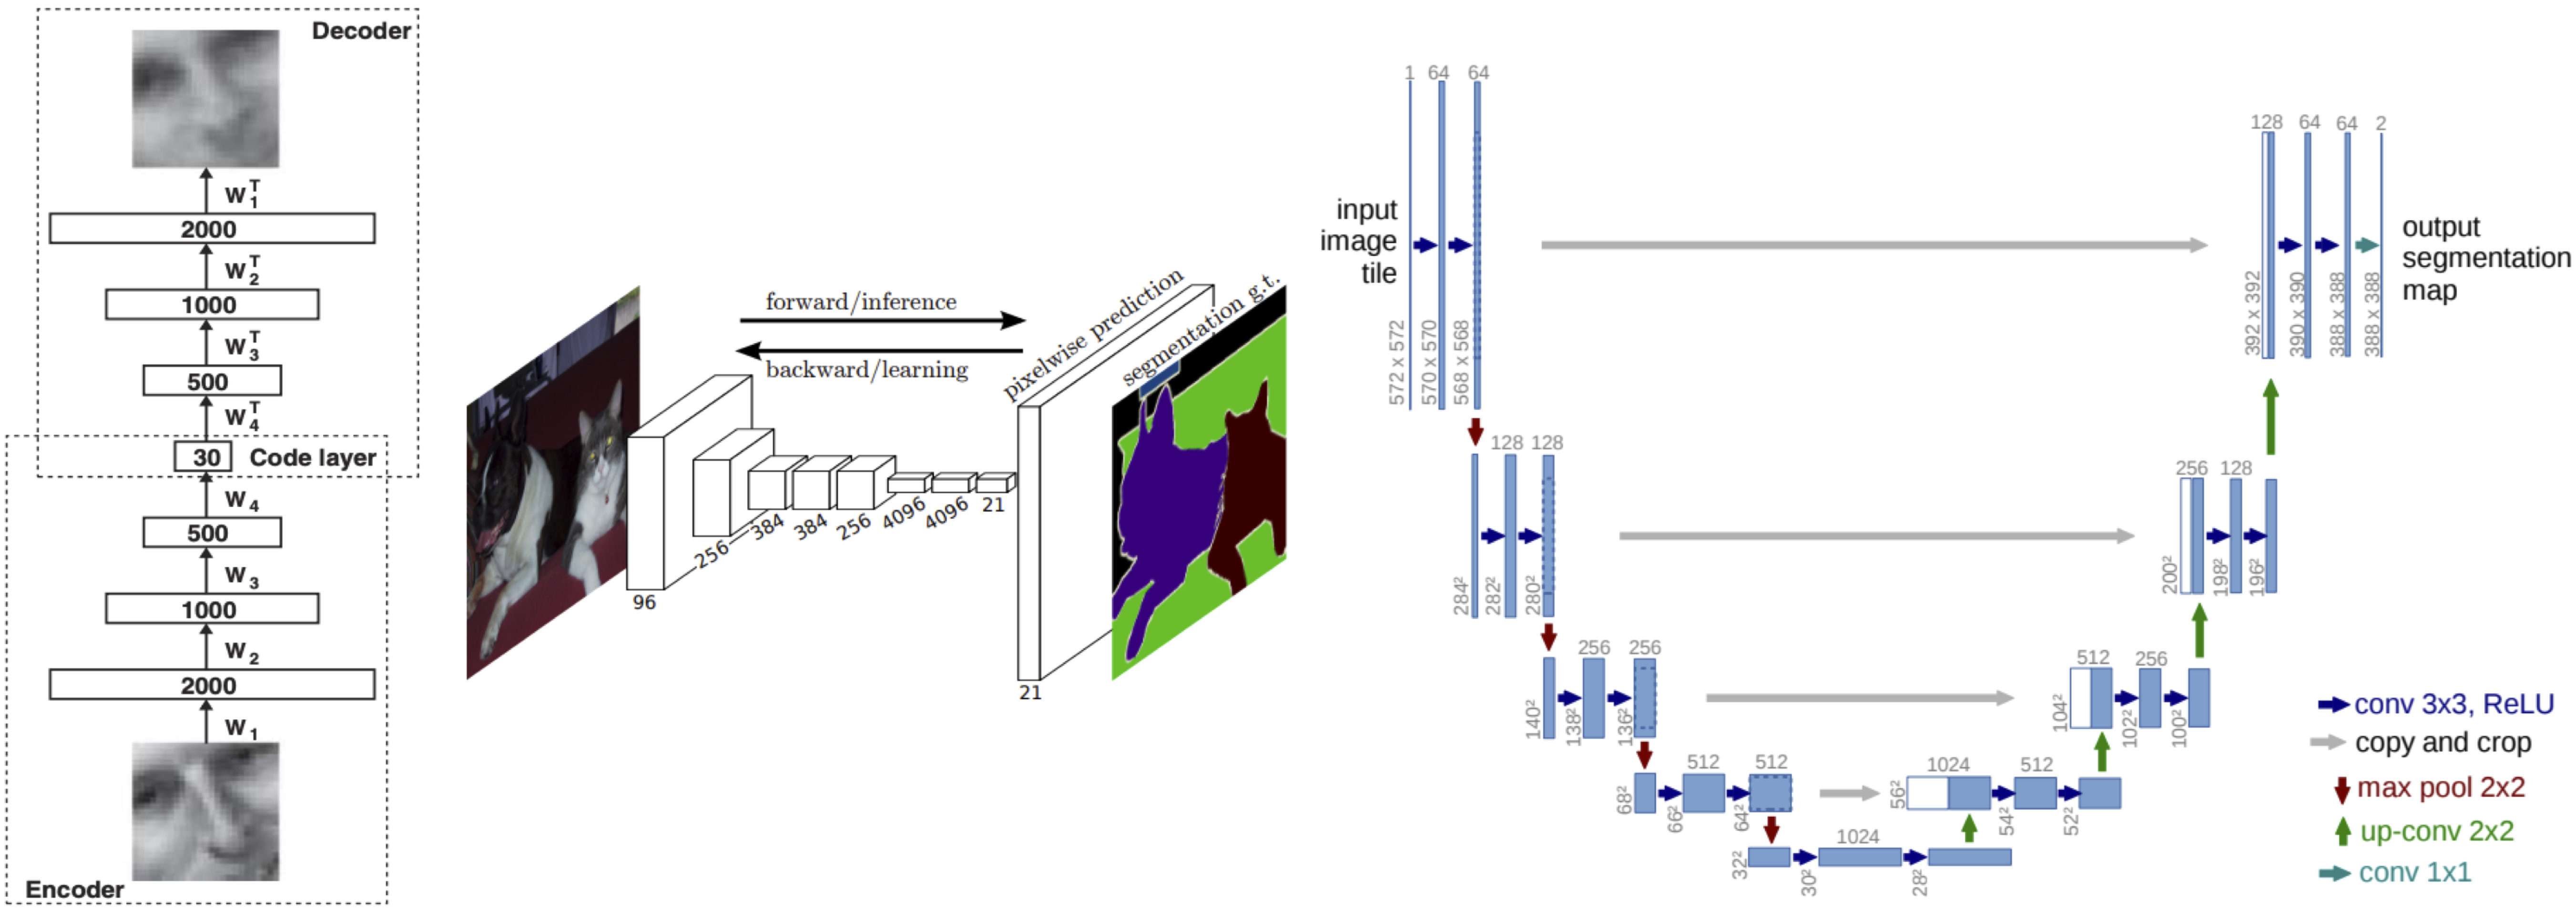
\includegraphics[width=1.0\textwidth]{figure/popular_encoder_decoder}
%	\caption{三种经典的编码器-解码器模型结构。从左到右依次为编码器-解码器~\cite{hinton2006reducing}、全CNN~\cite{long2015fully}和U-Net~\cite{ronneberger2015u}(图片均来自于原文)。} 
%	\label{fig:popular_encoder_decoder}
%\end{figure}

\begin{figure}[h!] % image examples & compare
	\centering
	\begin{subfigure}{0.22\textwidth}
		\centering
		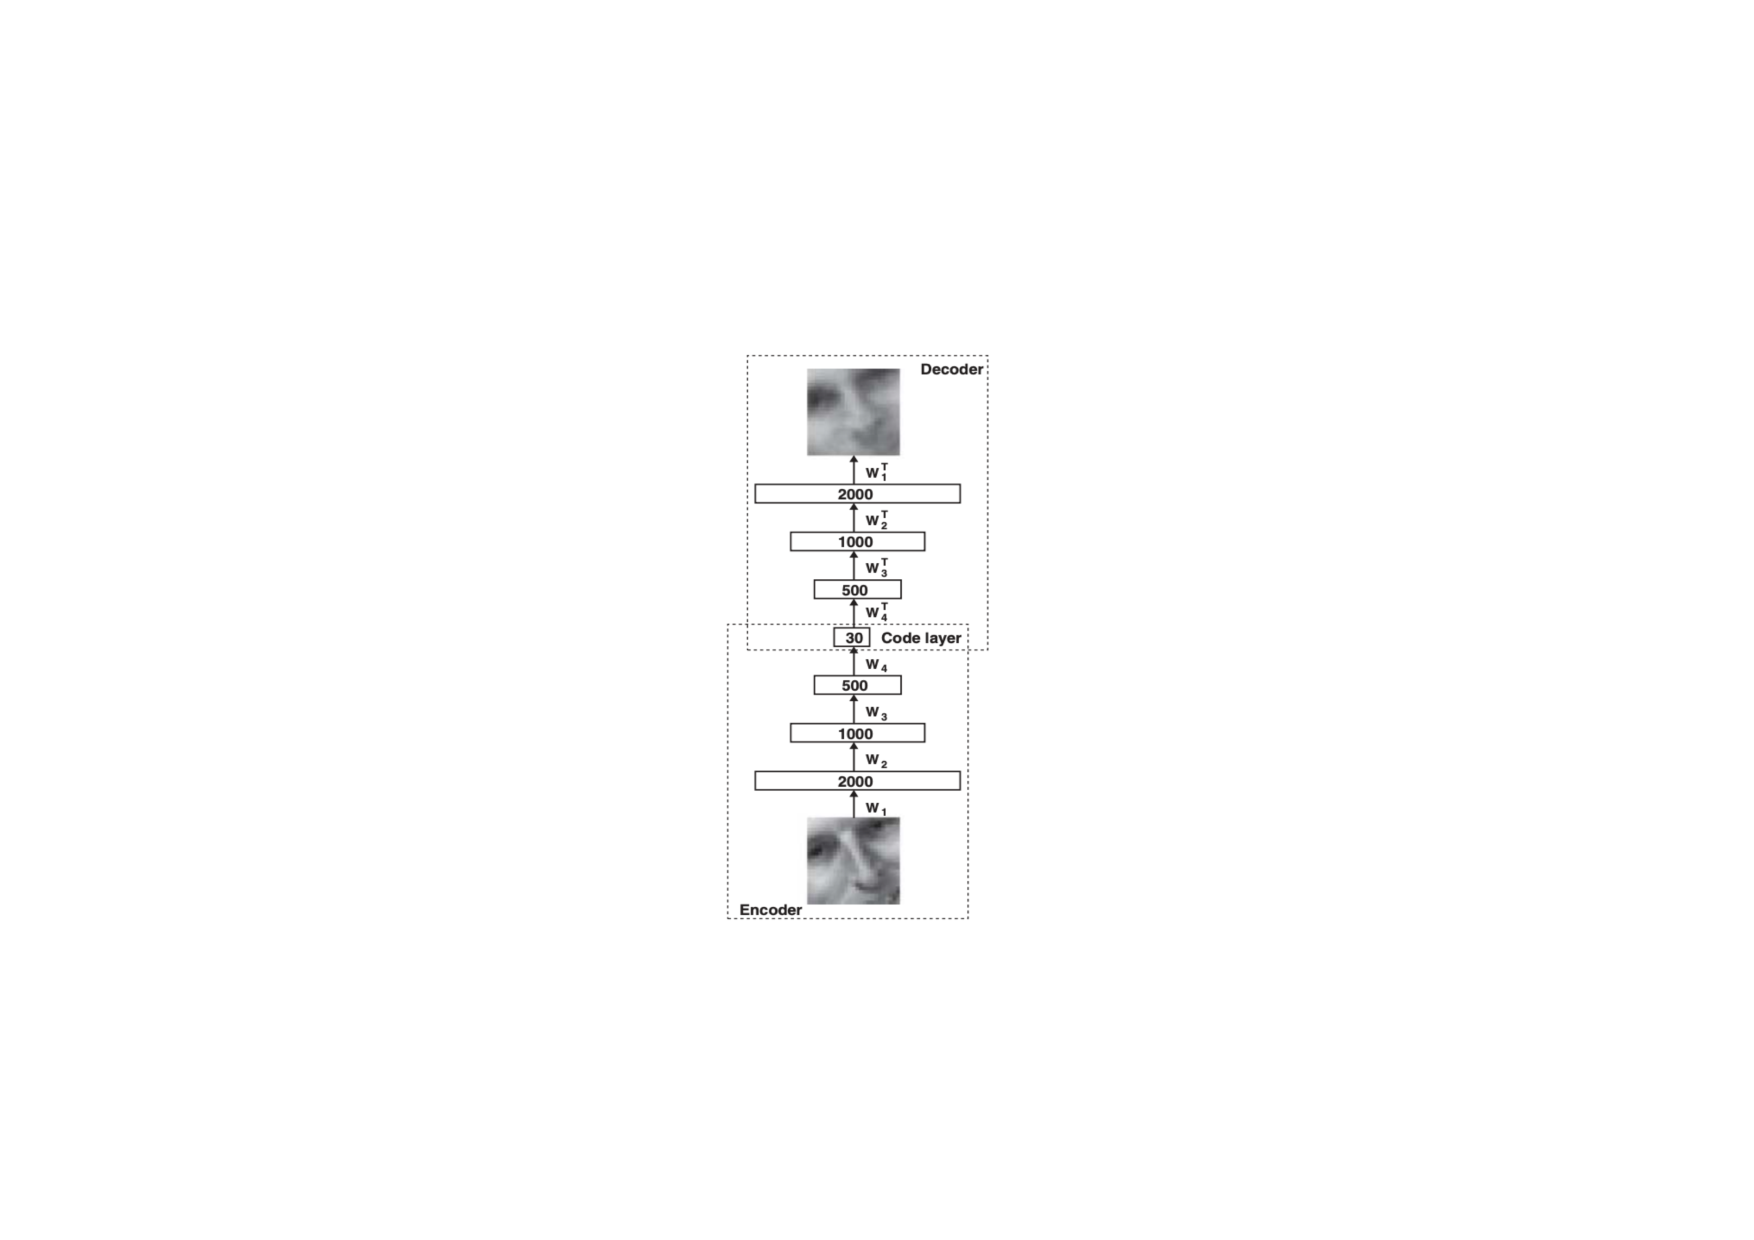
\includegraphics[width=1.0\textwidth]{figure/popular_encoder_decoder_original_encoder_encoder}
		\caption{Encoder-Decoder~\cite{hinton2006reducing}}
	\end{subfigure}
	\qquad
	\begin{subfigure}{0.71\textwidth}
		\centering
		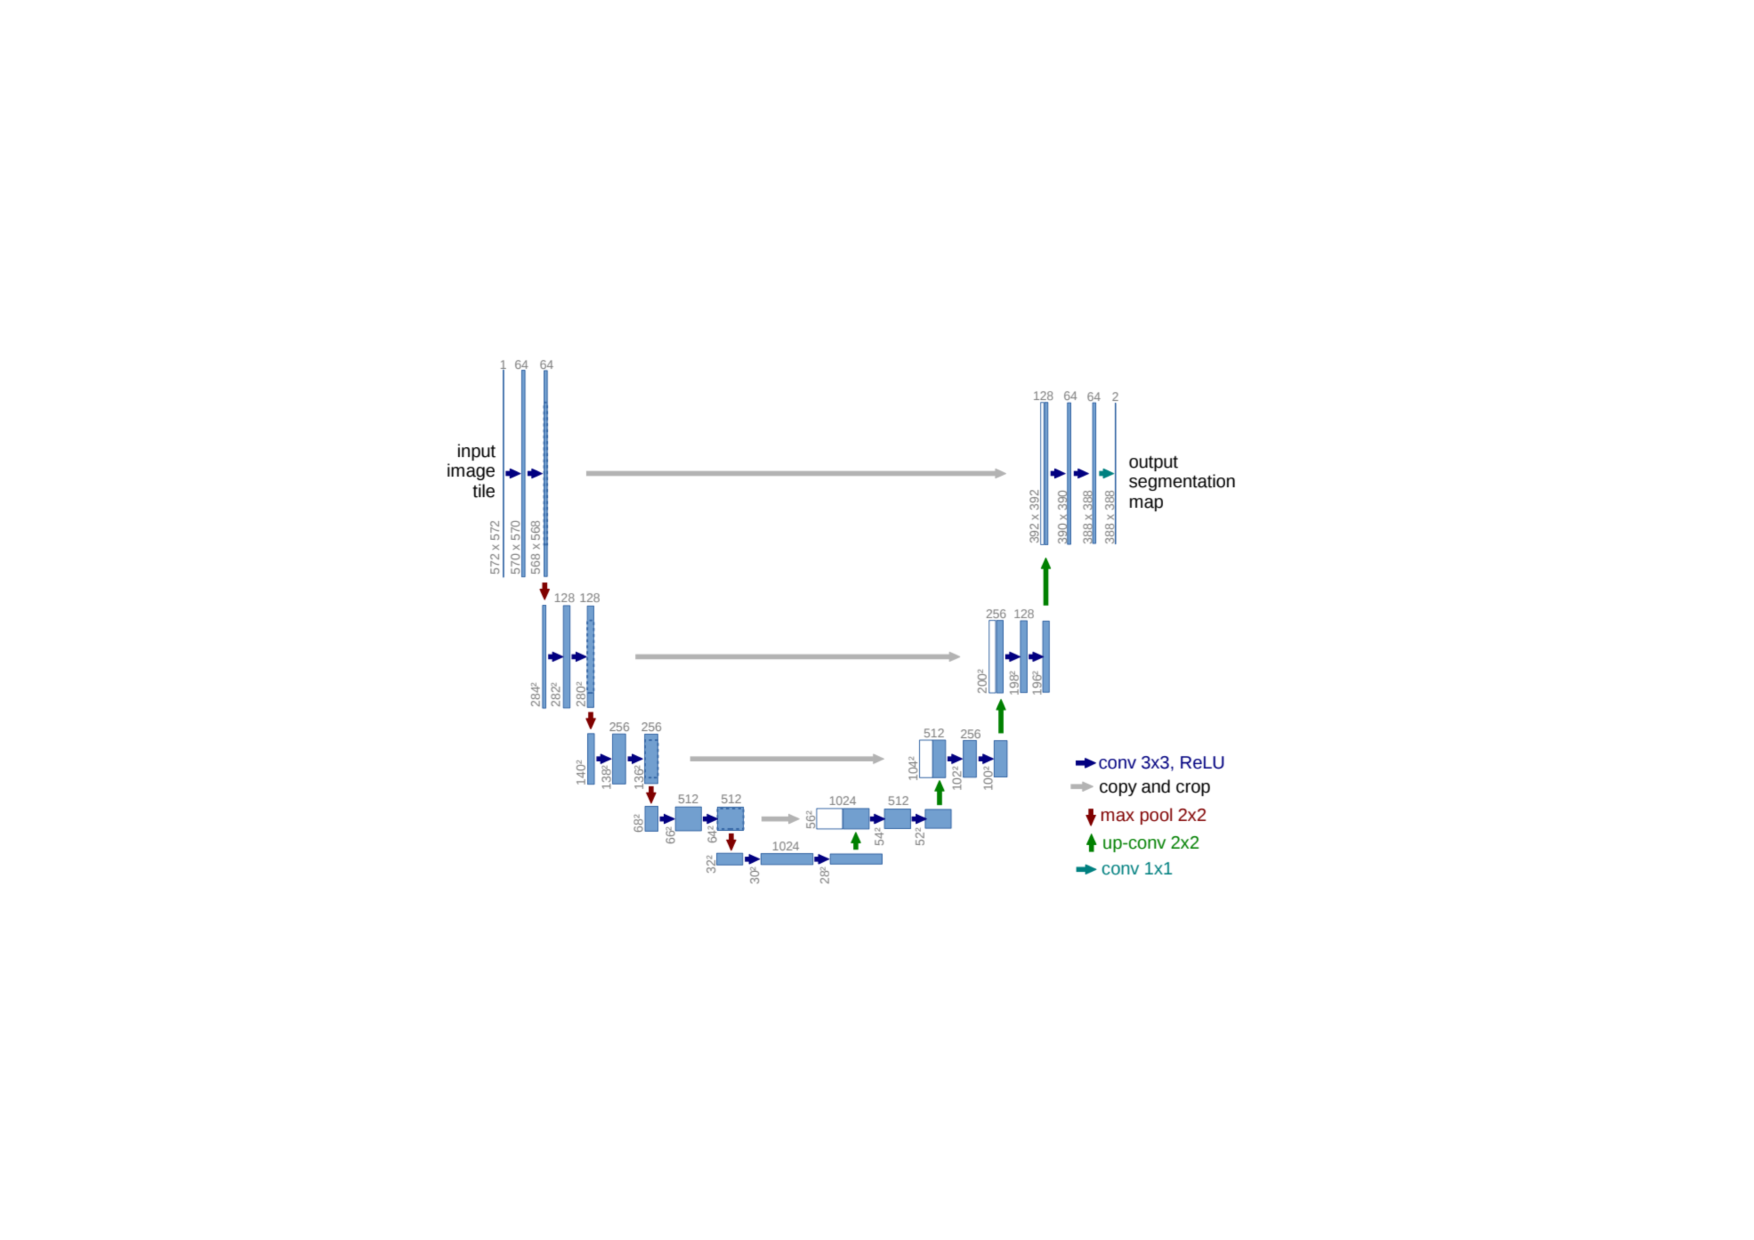
\includegraphics[width=1.0\textwidth]{figure/popular_encoder_decoder_unet}
		\caption{U-Net~\cite{ronneberger2015u}}
		\label{subfig:popular_encoder_decoder_unet}
	\end{subfigure}
	\caption[两种经典的编码器-解码器模型]{两种经典的编码器-解码器模型(图片均来自于对应论文~\cite{hinton2006reducing, ronneberger2015u})。} 
	\label{mulfig:popular_encoder_decoder}
\end{figure}

编码器-解码器自Hinton等人~\cite{hinton2006reducing}提出以来被广泛应用。编码器-解码器不是某一种网络,而是代表了一类网络。随后降噪编码器-解码器~\cite{vincent2008extracting}、稀疏编码器-解码器~\cite{coates2011analysis}、变分贝叶斯编码器-解码器~\cite{kingma2013auto}等不同用途的变体也相继被提出。编码器-解码器与CNN的结合启发了全卷积神经网络~\cite{long2015fully}、U-Net~\cite{ronneberger2015u}等经典网络结构。全卷积神经网络和U-Net均是图像分割任务(包括自然图像和医学图像)最为基础的网络结构。为了让读者对编码器-解码器模型结构有较为直观的认识,包括原始编码器-解码器和U-Net在内的两种经典网络结构如图\ref{mulfig:popular_encoder_decoder}所示。

在深度学学习领域,编码器-解码器是一种无监督的神经网络。从图\ref{mulfig:popular_encoder_decoder}可看出,编码器-解码器共同特点是由编码器和解码器组成:

1)编码器:编码器是不断将输入维度变小的过程,在传统神经网络中通常采用全连接层,而CNN一般会运用池化层实现下采样,不断减小输入维度,从而达到提取稀疏特征的目的。由于编码器可将输入维度不断降低,因此编码器-解码器最直观的应用便是图像压缩和图像去燥。在实际使用全卷积神经网络的过程中,为了让编码器在初始状态下就能提取到输入较好的特征表达,通常会利用深度学习网络知识可迁移的优点,用Image-Net~\cite{deng2009imagenet}上的预训练模型参数来初始化编码器~\cite{iglovikov2018ternausnet}。

2)解码器:解码器和编码器相反,是将输入尺寸不断扩大,最终恢复到原图像大小的过程。CNN通常会使用上采样或者反卷积~\cite{zeiler2010deconvolutional}操作以2倍关系逐步扩大输入维度,从而达到融合不同层次特征的目的。

本文使用到了U-Net~\cite{ronneberger2015u},故在此专门再介绍U-Net。除了以上特点之外,U-Net中还存在从编码器直接到解码器的跨层连接,这些跨层连接使网络可以将上下文信息传播到更高分辨率的层,使得特征融合更加充分。在网络可视化图上(见图\ref{subfig:popular_encoder_decoder_unet}),编码器和解码器相互对称,形成一个U型结构,这也是U-Net名称的由来。U-Net中只含有卷积层,不含任何全连接层,最后视不同任务而接上不同激活函数。U-Net启发了后续诸多优秀网络模型~\cite{zhou2018unet++, oktay2018attention, alom2019recurrent},
被广泛用于语义分割任务~\cite{cciccek20163d,dong2017automatic,li2018h}。

%被广泛用于语义分割任务~\cite{cciccek20163d, han2018framing, dong2017automatic, sevastopolsky2017optic, zhang2018ct}
%在医学影像领域更是大放异彩(比如图像重构~\cite{bhadra2020medical}、异常检测~\cite{Kohl2017AdversarialNF}、图像去噪~\cite{Yang2018LowDoseCI}和图像分割~\cite{Han2018SpineGANSS})。
%对抗生成网络(Generative Adversarial Networks,缩写为GAN)最初于2014年由Goodfellow等人~\cite{goodfellow2014generative}提出,就越来越受到学术界和工业界的重视。而随着GAN在理论与模型上的高速发展,GAN不仅在计算机视觉~\cite{zhu2017unpaired}、自然语言处理~\cite{qin2018dsgan}、人机交互~\cite{qiao2018emotional}等领域有着越来越深入的应用,还在医学影像领域大放异彩(比如图像重构~\cite{bhadra2020medical}、异常检测~\cite{Kohl2017AdversarialNF}、图像去噪~\cite{Yang2018LowDoseCI}和图像分割~\cite{Han2018SpineGANSS})。
\subsection{生成对抗网络}\label{subsec:gan_introduction}
生成对抗网络(Generative Adversarial Networks,缩写为GAN)最初于2014年由Goodfellow等人~\cite{goodfellow2014generative}提出,就受到学术界和工业界的重视。随着GAN在理论与模型上的高速发展,GAN不仅在计算机视觉~\cite{zhu2017unpaired}领域有着越来越深入的应用,还在医学影像领域大放异彩(比如,图像重构~\cite{bhadra2020medical}、异常检测~\cite{Kohl2017AdversarialNF}、图像去噪~\cite{Yang2018LowDoseCI}和图像分割~\cite{Han2018SpineGANSS})。GAN是生成式模型,由生成器和判别器组成,受博弈论中的零和博弈启发,GAN将生成问题视作判别器和生成器这两个网络的对抗和博弈。生成器努力生成新数据,判别器努力区分生成器生成的数据(一般记为“假”)和真实数据(一般记为“真”)。生成器尽量产生更真实的数据,而判别器尽量更完美地把真实数据与生成数据区分开来。由此,生成器和判别器形成对抗关系,彼此进步。在不断的迭代训练过程中,生成器生成的数据也就越来越逼近真实数据,即生成器学到的分布越来越接近真实数据代表的分布。在理想情况下,判别器无法区分生成器生成的数据和真实的数据。

设真实数据分布为$\ve{x}\sim p_{{data}}(\ve{x})$,噪音分布为$\ve{z}\sim p_{{z}}(\ve{z})$,$G$和$D$分别表示生成器和判别器。$\vv{\theta}_{g}$和$\vv{\theta}_{d}$分别表示生成器$G$和判别器$D$的训练参数。在GAN中,判别器被看做一个二类分类器,通常在器最后一层加上Sigmod激活函数,因而一般将交叉熵当做损失函数。判别器输出$D(\ve{x};\vv{\theta})$是一个数值,范围在$0$到$1$之间,表示样本来自于真实数据分布的可能性。运用最小最大优化理论,GAN的优化目标$V(D, G)$可写成:
\begin{eqnarray}\label{equ:gan_loss_func}
\min _{G} \max _{D} V(D, G)=\mathbb{E}_{ \ve{x} \sim {p}_{ {data }}(\ve{x})}[\log D(\ve{x};\vv{\theta})]+\mathbb{E}_{\ve{z} \sim {p}_{{z}}(\ve{z})}[\log (1-D(G(\ve {z};\vv{\theta});\vv{\theta}))].
\end{eqnarray}
\noindent 其中,$G(\ve {z};\vv{\theta})$表示生成器生成的数据样本。根据GAN的思想,通常先更新判别器,使判别器尽可能将来自真实数据分布的样本和来自生成器生成的数据分布的样本区分开来。随后更新生成器,使生成器生成的样本尽可能接近来自真实数据分布的样本,使得判别器无法区分样本来自真实数据分布还是生成器生成的数据分布。在实际训练时,一般采用判别器和生成器先后交替训练的策略:


1)固定生成器,更新判别器。这等价于用随机梯度上升算法最大化损失函数$L(\ve{x},\ve{z};\vv{\theta})$:
\begin{equation}
L(\ve{x},\ve{z};\vv{\theta})=\log D\left(\ve{x};\vv{\theta}\right)+\log \left(1-D(G(\ve{z};\vv{\theta}\right);\vv{\theta})).
\end{equation}
	
2)固定判别器,更新生成器。这等价于用随机梯度下降算法最小化损失函数$L(\ve{z};\vv{\theta})$:
	\begin{equation}
	L(\ve{z};\vv{\theta})=\log \left(1-D\left(G\left(\ve{z};\vv{\theta}\right);\vv{\theta}\right)\right).
	\end{equation}
%Kullback-Leibler散度~\cite{Kullback1951ONIA}或者Jensen-Shannon散度~\cite{Kantor2001FoundationsOS}

\noindent 以上朴素GAN中生成器和判别器均是多层感知机。在实际训练过程中存在参数量过大、训练困难、损失函数不具备可解释性、模式崩塌、容易出现梯度消失等问题,这些问题导致训练GAN经常失败。为了克服以上问题,各种改进模型相继提出,Alec等人~\cite{radford2015unsupervised}成功将CNN和GAN结合起来,提出了DCGAN,用CNN代替生成器和判别器中的多层感知机,使得训练GAN更加容易,生成图像的分辨率和质量也更高。针对训练过程中存在的梯度消失和模式崩塌问题,Martin等人~\cite{arjovsky2017wasserstein}提出了WGAN,使用Wasserstein-1距离代替素朴GAN~\cite{goodfellow2014generative}中使用的Kullback-Leibler散度\footnote{https://en.wikipedia.org/wiki/Kullback\%E2\%80\%93Leibler\_divergence}或者Jensen-Shannon散度\footnote{https://en.wikipedia.org/wiki/Jensen\%E2\%80\%93Shannon\_divergence},并且采用权值截断(Weight Clipping)满足利普希茨连续条件\footnote{https://en.wikipedia.org/wiki/Lipschitz\_continuity}(Lipschitz Continuity),但这也会造成训练参数趋向两个截断阈值,导致GAN不容易收敛。为了更好满足利普希茨连续条件,Ishaan等人~\cite{gulrajani2017improved}采用梯度惩罚项(Gradient Penalty),提出了WGAN-GP。WGAN-GP可以有效避免GAN训练过程中的梯度消失问题,其训练过程也比较稳定,网络收敛得也较快。此外,Wasserstein-1距离还对训练过程有指示作用,Wasserstein-1距离越接近0,表示WGAN-GP训练得越好。故本文提出的模型中的GAN采用WGAN-GP。与朴素GAN~\cite{goodfellow2014generative}不同的是,在WGAN-GP中,判别器不再被看作二分类器,而是近似去拟合Wasserstein-1距离,属于回归任务,因此判别器最后一层也不再有Sigmoid激活函数。设$\ve{y}\sim {p}_{g}(\ve{y})$表示给定噪音分布$\ve{z}\sim {p}_{{z}}(\ve{z})$时生成器所代表的数据分布。再加上梯度惩罚项,WGAN-GP的优化目标$L(\ve{x},\hat{\ve{x}},\ve{y};\vv{\theta})$可写作:
\begin{equation}\label{wgan_gp_loss_func}
  \begin{aligned}
	L(\ve{x},\hat{\ve{x}},\ve{y};\vv{\theta})=&\mathbb{E}_{\ve{y} \sim {p}_{{g}}}[D(\ve{y};\vv{\theta})]-\mathbb{E}_{\ve{x} \sim {p}_{{data}}}[D(\ve{x};\vv{\theta})] \\ &+\lambda \mathbb{E}_{\hat{\ve{x}} \sim {p}_{\hat{{x}}}}\left[\left(\left\|\nabla_{\hat{\ve{x}}}D(\hat{\ve{x}};\vv{\theta})\right\|_{2}-1\right)^{2}\right].
  \end{aligned}
\end{equation}
其中,$\lambda$为梯度惩罚项的权重,注意此处分布${p}_{\hat{{x}}}$不是对整个样本空间采样,而只对分布${p}_{{data}}$和分布${p}_{{g}}$之间的空间采样。与朴素GAN的损失函数相比,判别器的损失函数不再取$\log$,这是因为WGAN-GP损失函数中不再使用Kullback-Leibler散度或者Jensen-Shannon散度。在训练WGAN-GP时,判别器和生成器同样先后交替训练:

1)固定生成器,更新判别器。这等效于最小化损失函数$L(\ve{x},\ve{z};\vv{\theta})$:
\begin{equation}
\begin{aligned}
	L(\ve{x},\ve{z};\vv{\theta})=D({{\ve{y}}};\vv{\theta})-D({\ve{x}};\vv{\theta})+\lambda\left(\left\|\nabla_{\hat{\ve{x}}} D(\hat{\ve{x}};\vv{\theta})\right\|_{2}-1\right)^{2}
\end{aligned}
\end{equation}

2)固定判别器,更新生成器。这等效于最小化损失函数$L(\ve{z};\vv{\theta})$:
\begin{equation}
	L(\ve{z};\vv{\theta})=-D\left(G(\ve{z};\vv{\theta})\right).
\end{equation}
\noindent 到此,生成对抗网络的基本理论介绍结束。下一节介绍可定位疾病标记物的相关方法。
\section{疾病标记物定位方法}\label{sec:related_work}
随着计算机技术在医学影像领域的广泛应用,目前已有可用于疾病标记物定位的相关方法提出,主要有多示例学习(Multiple Instance Learning,缩写为MIL)、CNN可视化方法和弱监督目标定位。本小节将详细介绍这三种思路中的部分经典方法,重点突出这些方法处理疾病标记物定位任务时的优势和劣势。
\subsection{多示例学习}
MIL是由Maron等人~\cite{maron1998framework}提出,是一种与监督学习、半监督学习和非监督学习有所不同的不确切监督,也可用于处理弱监督问题。在处理图像数据时,MIL方法可通过训练一个二分类器,不仅完成对图像数据的分类任务,还能粗略定位图像数据中的的显著性区域,这在诸如没有细粒度标记训练数据的感兴趣区域定位的任务中特别有用。

MIL中是以多示例包(Bag)为训练单元,训练集是由许多具有分类标签(Label)的多示例包组成,每个多示例包含有若干个没有分类标签的示例(Instance)。如果多示例包至少含有一个正示例,则该包被标记为正类多示例包(正包)。如果多示例包的所有示例都是负示例,则该包被标记为负类多示例包(负包)。以图像是正常还是异常为例,通常将异常图像看作是正包,将正常图像看作是负包。设$\ve{X}=\{\ve{x}_1,\ve{x}_2,...,\ve{x}_N\}$,其中每一个$\ve{x}_i$均是从图像中相应第$i$个区域中提取出来的特征向量,$N$是图像被分割出的区域(示例)个数。拿二类问题来说,设示例${\ve{x}_1}$,$\ve{x}_2$,...,$\ve{x}_N$对应的标签为${y_1}$,${y_2}$,...,${y_N}$。则包$\ve{X}$的标签$y\in \{-1,+1\}$可用形式化语言定义为:
\begin{equation}
y=\left\{\begin{array}{ll}
{+1} & {\text { if } \quad \exists {y}_{i}: {y}_{i}=+1;} \\
{-1} & {\text { if } \quad \forall {y}_{i}: {y}_{i}=-1.}
\end{array}\right.
\end{equation}
%https://link.springer.com/content/pdf/10.1007%2F978-3-319-07998-1_65.pdf
其中,$+1$和$-1$分别表示正包和负包。对于图像问题,根据MIL思想,将单张图像看作一个示例包,再对单张图像进行分块操作得到许多小方块,再将这些小方块看作一个个示例。多示例学习的目的是,通过对具有分类标签的多示例包的学习,建立多示例分类器,并将该分类器应用于未知多示例包的预测。MIL的目标是找到正包的原型,换句话说,找出所有正包的共同点。随后,在示例空间中,找出最能表现原型的示例。MIL也在医学图像处理领域得到广泛应用,可解决医学影像领域中的诸多问题,比如,眼底图像中的玻璃疣定位~\cite{lu2015effective}、X射线图像中肺结核诊断与病灶区域定位~\cite{melendez2014novel}、皮肤镜图像中蓝白结构结构定位~\cite{madooei2018learning}、病理图像中前列腺癌诊断与病灶区域定位~\cite{campanella2018terabyte},眼底图像中的视网膜神经纤维分割~\cite{manivannan2017subcategory}和数字病理图像中的癌症诊断~\cite{kandemir2014empowering}。

但是这种方法存在诸多缺点,首先对单张图像进行分块不易操作,分块尺寸过大时,示例中很可能会包括较多正常区域,导致精确度不够;反之,当分块尺寸过小时,会产生过多示例,这将大大增大后续训练的计算复杂度和计算量。因此,MIL方法只适合用于粗略定位图像中的目标物(例如,疾病标记物)。此外,当处理多类问题时,示例包就会出现多标签,使得问题的复杂度大大增加,造成分析的难度太大。因此,与其在算法和应用上的繁荣发展相反,近些年来,这种思路少有人问津。
%~\cite{gondra2014object, wu2015deep,Maron1998MultipleInstanceLF}也非常少。

\subsection{卷积神经网络的可视化}\label{subsec:visulization_methods}
CNN在图像分类、语音识别、自然语言处理等大规模任务中的取得了相当大的成就,使其成为先进的人工智能系统中最受欢迎的工具。尽管只能将成功的部分原因归功于这种网络的训练过程中算法的进步,但是学习过程和所学内容的内在性仍然很模糊,即CNN一直是个“黑匣子”,我们始终不知道其内部运行机制,更无法得知其作出判断的背后依据。然而,CNN所做决定的依据很多时候与所做决定同样重要,比如,在医学领域,如果医生看不到人工智能系统给出诊断方法,医生也就无法接受人工智能系统所给提出的对患者的治疗方案。因此,我们需要有一种方式了解导致CNN失败或成功的原因。如果我们无法解释模型的工作原理,我们也就无法信任模型的给出的结果与判断。更重要的是,较差的网络可解释性极大地阻碍了对各个网络层的鲁棒性评估,进一步优化网络结构,以及对不同应用的网络适应性和可移植性,这也是CNN的可视化需要回答的直接动力和实际意义。
\begin{table}[h]
	% reference: https://arxiv.org/pdf/1804.11191.pdf
	\centering
	\caption[四类有代表性的CNN可视化方法]{四类有代表性的CNN可视化方法。}
	\label{tab:typical_visualization_methods}
	\begin{tabular}{c|c|c}
		\toprule[2pt]
		方法 & 解释粒度 & 代表工作 \\ \midrule[2pt]
		激活最大化方法 & 网络层  & Simonyan等人~\cite{simonyan2013deep}  \\\hline
		%反卷积网络 & 网络层  & Zeiler等人~\cite{zeiler2014visualizing, zeiler2010deconvolutional, zeiler2011adaptive} \\\hline
		基于梯度的可视化方法 &  神经元 & Selvaraju等人~\cite{selvaraju2017grad},Springenberg等人~\cite{springenberg2014striving} \\  \hline
		网络逆转 & 网络层 &Mahendran等人~\cite{mahendran2015understanding, mahendran2016visualizing},Dosovitskiy等人~\cite{dosovitskiy2016inverting}\\
		\bottomrule[2pt]
	\end{tabular}
	\label{tab:four_visulization_types}
\end{table}
%除此之外,还能通过t-SNE方法~\cite{maaten2008visualizing}对图像的特征向量进行降维操作,以在低维空间中查看数据的宏观分布。除此之外,还能对图像的特征向量进行降维操作,以在低维空间中查看数据的宏观分布。
CNN的可视化问题自提出以来,有很多研究者提出了解决方法。最简便也是最直接的方法是利用PyTorch\footnote{https://pytorch.org/}、TensorFlow\footnote{https://www.tensorflow.org/}等工具直接观察其网络结构可视化图,查看卷积核大小、卷积层输入和输出尺寸、卷积层参数等相关信息。另一种可视化技术是获取大型数据集,通过网络输入图像,并跟踪哪些图像最大程度地激活了某些神经元。然后,我们可以将图像可视化,以了解神经元在其感受野中正在寻找什么,Girshick等人~\cite{girshick2014rich}提出了这样一种可视化技术,用于精确的对象检测和语义分割。因为ReLU神经元本身不一定具有任何语义,所以这种方法只有输入特征图沿着与过滤器权重相对应的轴方向的可视化结果。Zeiler等人~\cite{zeiler2014visualizing}提出的方法可以更为直接的了解到神经元真正感兴趣的区域或者物体,通过依次遮挡图像每一部分来绘制感兴趣类别的概率与遮挡物位置的关系图。以上可视化方法主要关注浅层特征,对CNN工作机制的解释能力有限。随着CNN的快速发展和实现,可视化已被扩展到解释CNN的整体工作机制,解释粒度也越来越细化。表\ref{tab:typical_visualization_methods}回顾了三类有代表性的可视化方法。
\subsubsection*{激活最大化方法}
激活最大化(Activation Maximization)是一种通过合成特定输入图像,从而最大化在任意层中的特定神经元激活的方法。最初是由Erhan等人~\cite{erhan2009visualizing}提出的,被用于深度置信网络~\cite{hinton2006fast}高层神经元的可视化。随后,Simonyan等人~\cite{simonyan2013deep}将其扩展,用于解释CNN。以多分类问题为例,设$\ve{s}_{c}(\ve{x})(0\leq \ve{s}_{c}(\ve{x}) \leq 1)$表示为输入图像$\ve{x}$被CNN分到类别$c$的分数,使用L-2范数作为正则化项,则激活最大化方法用于解释CNN的目的在于重建类别$c$对应的原型图$\ve{x^*}$,使得$\ve{s}_c$最大,激活最大化方法可形式化为:
%设输入图像为$\ve{x}$,模式图像为$\ve{x}^*$,可形式化表示为:
%\begin{equation*}
%x^{*}=\underset{x}{\operatorname{argmax}}\left(a_{i, %l}(\theta, x)-\lambda(x)\right).
%\end{equation*}
%其中,$\theta$表示网络参数,
%$S_{c}(x)(0\leq S_{c}(x) \leq 1)$是经过Softmax激活函数得到的类别分数,
\begin{equation}
\ve{x}^*=\underset{\ve{x}}{\operatorname{arg\,max}}( {\ve{s}}_{c}(\ve{x})-\lambda\|\ve{x}\|_{2}^{2}).
\end{equation}
注意,正则项有多种选择,L-2范数通常会将图像平滑。高斯模糊也是常见的正则项,通常会抑制图像中的高频信息。此类方法通常都会固定网络参数,只是根据反向传播算法不断更新输入图像$\ve{x}$,从而合成具有特定模式的输入图像,得到类别$c$的原型图$\ve{x}^*$。
%\subsubsection{反卷积网络}
%\begin{figure}[h]
%	\centering
%	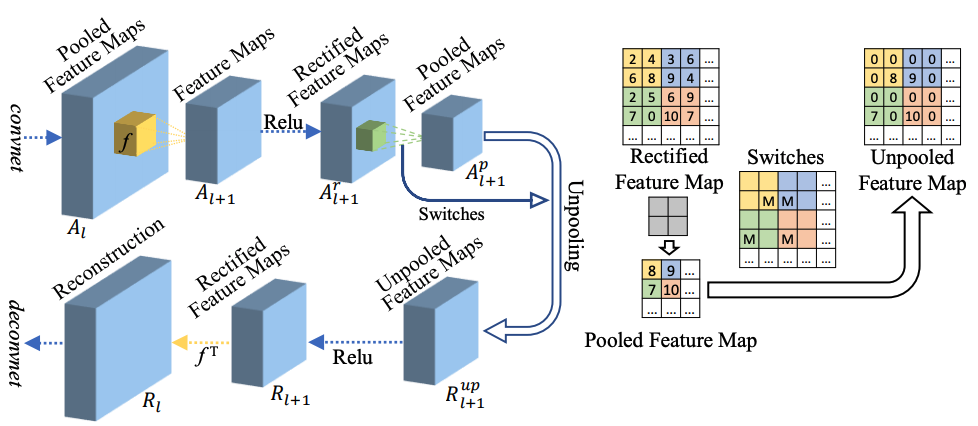
\includegraphics[width=1.0\textwidth]{figure/deconvnet_architecture}
%	\caption{DeconvNet模型结构图(图片来自于原文)。}
%	\label{fig:deconvnet_architecture}
%\end{figure}
%激活最大化方法从最大化特定神经元的激活来解释CNN。反卷积网络(DeconvNet)~\cite{zeiler2014visualizing, zeiler2010deconvolutional, zeiler2011adaptive}从输入图像的角度解释了CNN。它从输入图像中找到激活卷积层中特定神经元的选择性模式。通过将低维神经元的特征图逐层映射回原始图像尺寸来重建图像。这个投影这个过程由反卷积网络实现,这种网络包含反卷积层、反池化层、反ReLU激活函数等逆运算。基于DeconvNet的可视化并不仅仅是分析神经元的兴趣,而是展示了一种直接的特征分析方法。DeconvNet模型结构图如图\ref{fig:deconvnet_architecture}所示,可以发现,DeconvNet是CNN网络的逆过程,CNN中存在的操作在DeconvNet中均有对应逆操作。DeconvNet将图片特征从特征空间转化到像素空间,以发现是哪些像素激活了特定的特征,达到分析解释CNN的目的。另外,用DeconvNet还有可用于可视化一个已经训练好的网络模型,无须没有学习训练的优点。所以DeconvNet使用起来比较简单。
\subsubsection*{基于梯度的可视化方法}
梯度是CNN中非常重要的概念,CNN在前向传播阶段计算损失。回传的过程,实质上是梯度的计算和根据梯度更新训练参数的过程。不难理解,流过某个神经元的梯度越大,则代表前向传播时该神经元激活值越大,说明该神经元越重要。基于梯度的网络可视化方法就是充分利用CNN中流动的梯度,从梯度角度来解释每一个神经元在网络中所起到的作用,相对上述激活最大化方法,基于梯度的方法可得到更为精细的可视化结果。另外,CNN每一层中的每个神经元均有梯度,因而基于梯度的方法还更为灵活,可以实现位于任意层的任意神经元的可视化。在本小节,我们将介绍三种基于梯度的可视化方法:反卷积网络~\cite{zeiler2010deconvolutional}、Guided-Backpropagation~\cite{springenberg2014striving}和Grad-CAM~\cite{selvaraju2017grad}。

反卷积网络引入了卷积操作的逆运算反卷积。反卷积将特征空间映射回像素空间,来揭示什么样的输入模式能够产生特定的输出特征,但是这种方法也会额外引入物体以外的噪声。为了避免这一问题,对于ReLU反向传播,与一般梯度回传法则不同的是,Guided-Backpropagation组合了反卷积网络~\cite{zeiler2010deconvolutional}和一般梯度回传中ReLU函数梯度计算法则。此外,Guided-Backpropagation还用带步长的卷积层(如步长为2,卷积核为$3\times 3$的卷积层也可达到输入尺寸减半的效果)代替池化操作,使得Guided-Backpropagation不仅可以得到更为精细、细节更为丰富的可视化结果,还能可视化高层的特征(在这种情况下,反卷积网络可视化经常会失效)。
\begin{figure}[h]
	\centering
	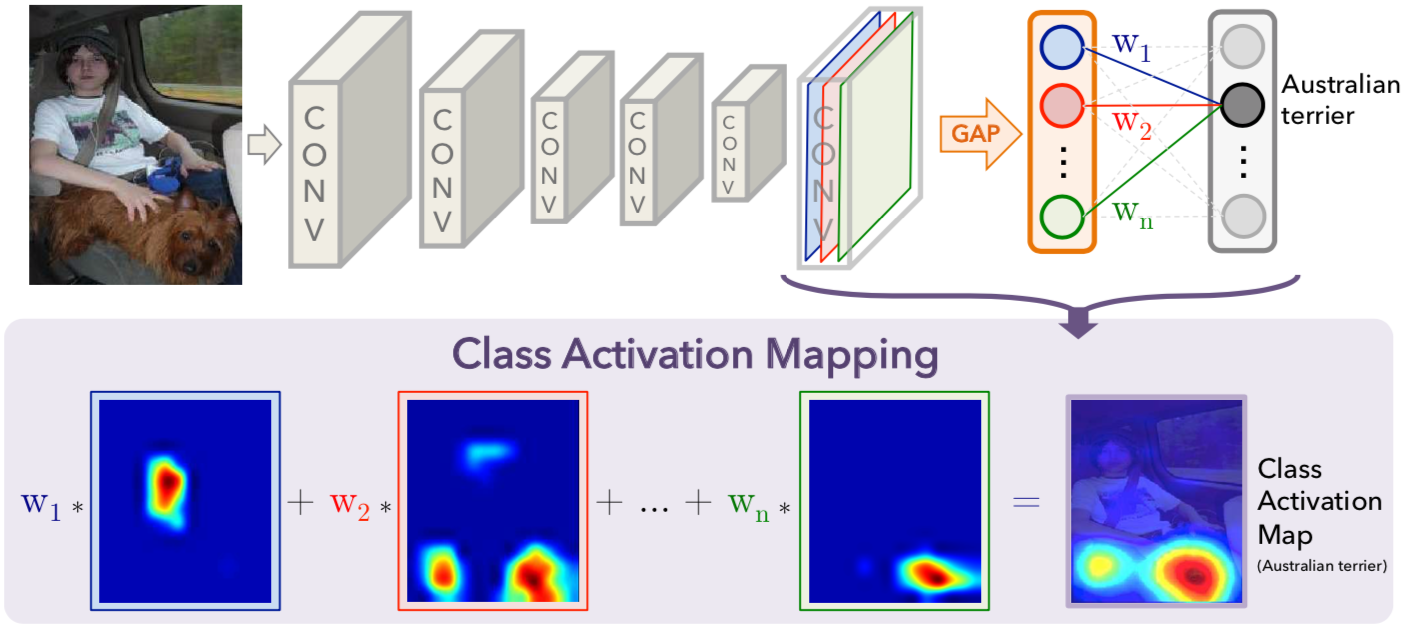
\includegraphics[width=1.0\textwidth]{figure/cam_arichitecture}
	\caption[CAM可视化]{CAM可视化(图片来自于对应原文~\cite{zhou2016learning})。}
	\label{fig:cam_arichitecture}
\end{figure}
%\begin{figure}[h]
%	\centering
%	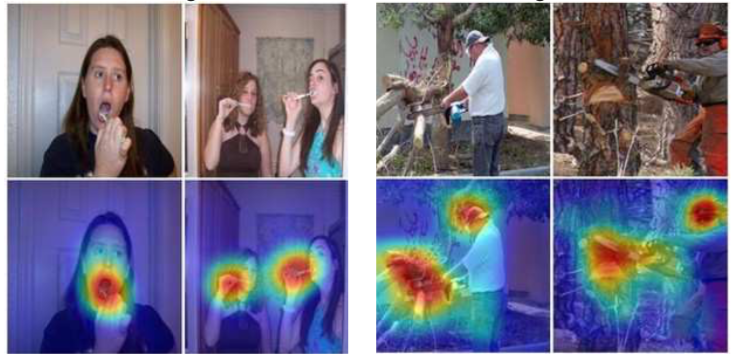
\includegraphics[width=1.0\textwidth]{figure/cam_example}
%	\caption{CAM可视化效果图示例(图片来自于原文)。}
%	\label{fig:cam_example}
%\end{figure}
%\vspace{-1.5cm}
\begin{figure}[h]
	\centering
	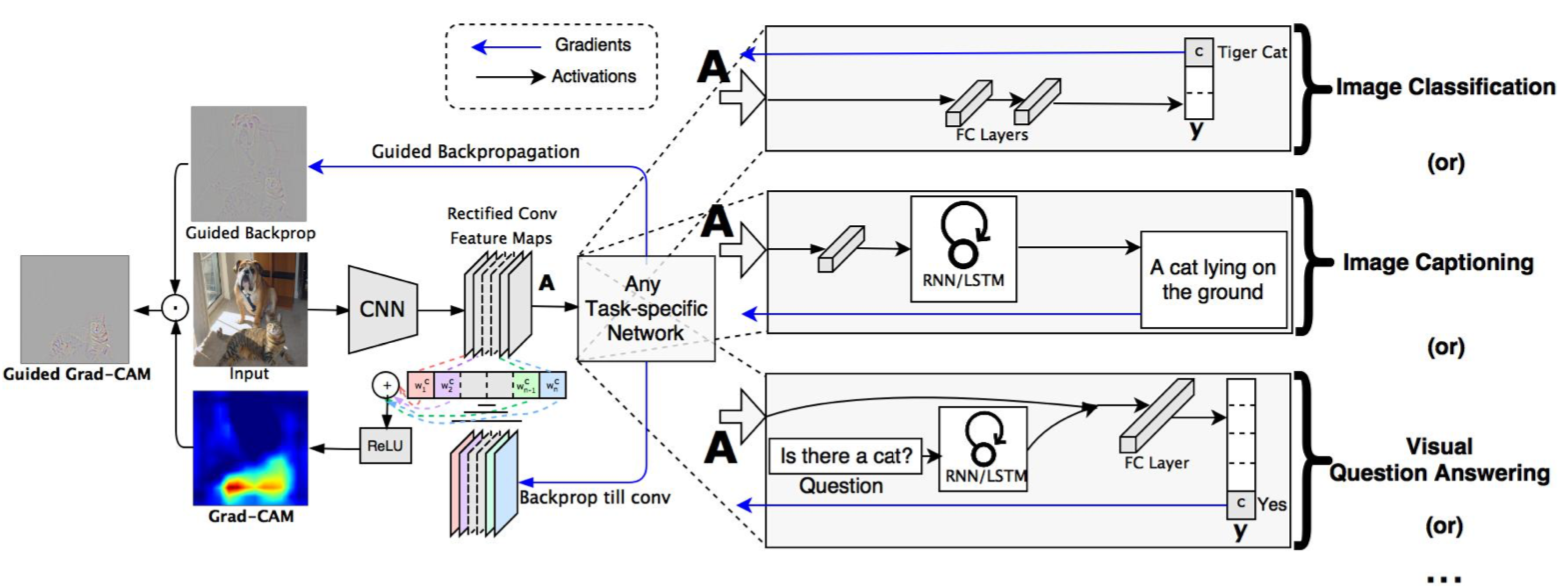
\includegraphics[width=1.0\textwidth]{figure/grad_cam_architecture}
	\caption[Grad-CAM可视化]{Grad-CAM可视化(图片来自于对应原文~\cite{selvaraju2017grad})。}
	\label{fig:grad_cam_architecture}
\end{figure}
%\begin{figure}[h]
%	\centering
%	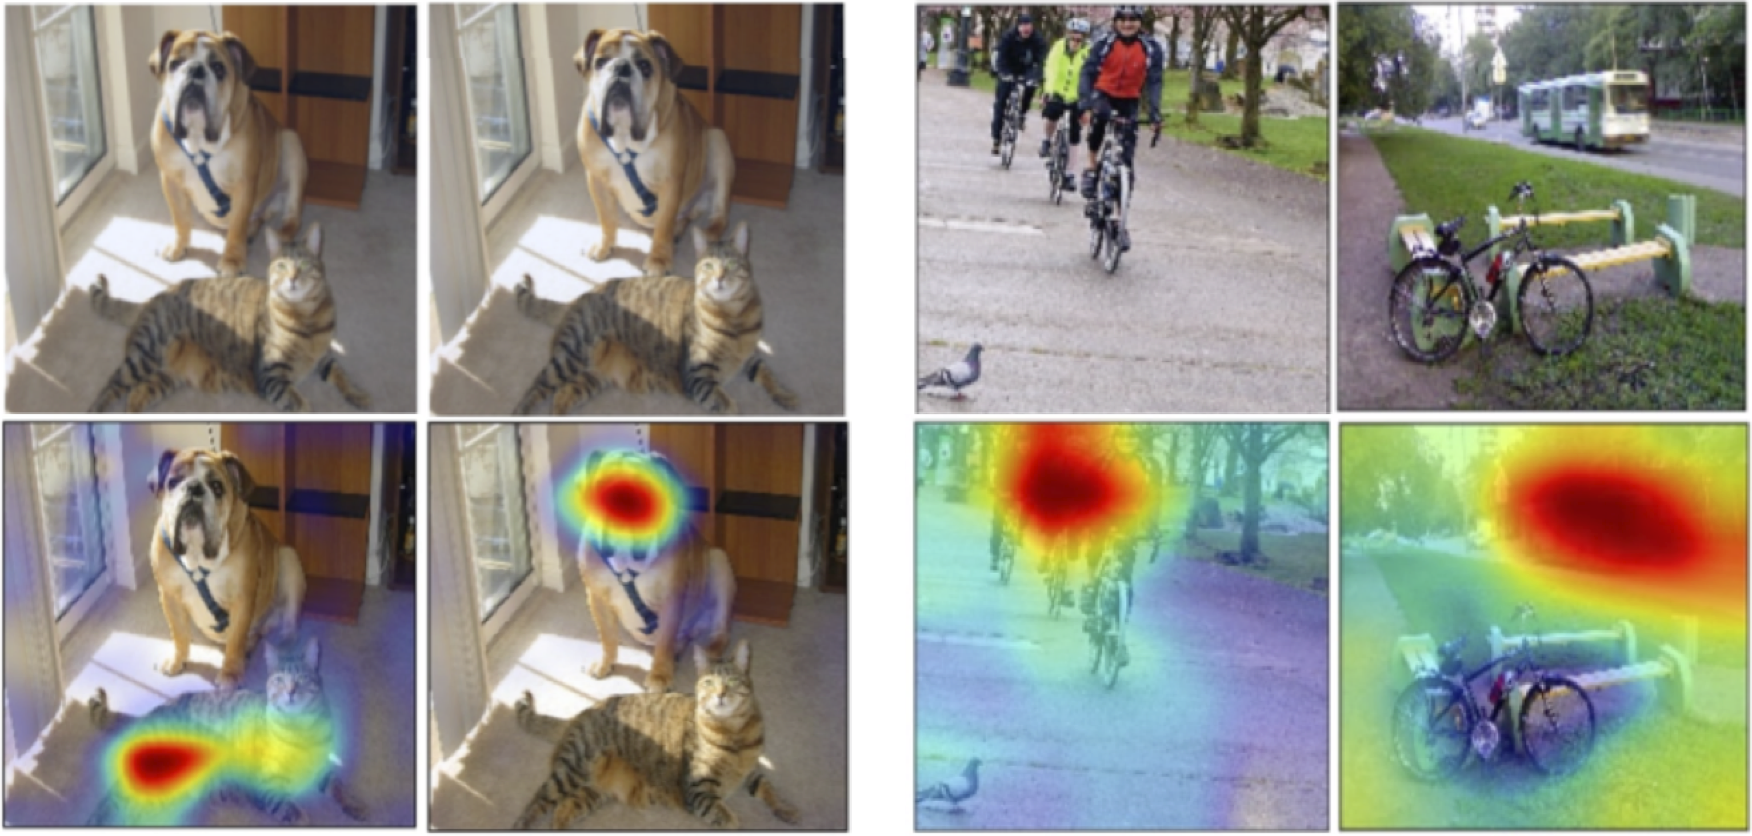
\includegraphics[width=1.0\textwidth]{figure/grad_cam_example}
%	\caption{Grad-CAM可视化效果图示例(图片来自于原文)。} 
%	\label{fig:grad_cam_example}
%\end{figure}
另外一种基于梯度,应用极为广泛的可视化方式是Grad-CAM,由于Grad-CAM是基于CAM~\cite{zhou2016learning}的。在此,先来介绍CAM。如图\ref{fig:cam_arichitecture}所示,全局均值池化(Global Average Pooling,缩写为GAP)输出最后一个卷积层每个单元的特征图的空间平均值,这些值的加权和用于生成最终输出。同样,我们计算最后一个卷积层的特征图的加权和,便可以得到类激活图(Class Activation Map)。下面我们以多分类问题($N$表示类别个数)为例进行更为详细的描述(假设最后一层激活函数是Softmax)。对于给定的图像,令$\ve{F}_k(x, y)$表示激活空间位置最后一个卷积层中第$k$个特征图的$(x,y)$位置的激活值。对于第$k$个特征图执行GAP,则GAP结果$\hat{\ve{F}}_k=\sum_{x, y} \ve{F}_{k}(x,y)$。因此,对于类别$c$,被送到Softmax激活函数的输入$\ve{s}_c=\sum_{k} \ve{W}_{k}^{c} \ve{F}_{k}$,其中$\ve{W}_k^c$是第$k$个特征图对应于类别$c$的权重。实质上,$\ve{W}_{k}^{c}$还可表示第$k$个特征图对于类别$c$的重要性。故这张图像被判断为类别$c$的概率${\ve{p}}_c$(经过Softmax激活函数)可定义为$\ve{p}_c=\frac{\exp \left(\ve{s}_{c}\right)}{\sum_{i=1}^{i=N} \exp \left(\ve{s}_{i}\right)}$。根据以上定义,我们可以作出如下推导:
\begin{equation}
\ve{s}_{c}=\sum_{k} \ve{W}_{k}^{c} \sum_{x, y} \ve{F}_{k}(x, y)=\sum_{x, y} \sum_{k} \ve{W}_{k}^{c} \ve{F}_{k}(x, y).
\end{equation}
我们定义$\ve{M}_c$为类别$c$的类激活图,则:
\begin{equation}\label{equ:cam_heatmap_compute}
\ve{M}_{c}(x, y)=\sum_{k} \ve{W}_{k}^{c} \ve{F}_{k}(x, y).
\end{equation}
不难发现,$\ve{M}_{c}(x, y)$直接表明了空间位置$(x,y)$处的激活值对于该图像被分为类别$c$的重要性程度。注意CAM在网络最后一层是GAP的情况下方能使用,例如,CAM不能实现对VGG-19~\cite{simonyan2014very}的可视化。为此,Grad-CAM计算类激活图的特征加权系数不是分类器的权值,而是通过反向传播计算的梯度,因此Grad-CAM适用于任何CNN中,其网络结构如图\ref{fig:grad_cam_architecture}所示。Grad-CAM与CAM相比,它的优点是适用的范围更广,可以认为是CAM的泛化,Grad-CAM可以应用到各种任务(比如,CNN可视化和弱监督图像分割)。本文将这两种方法用于弱监督条件下的疾病标记物定位。Grad-CAM还能与Guided-Backpropagation结合,可得到更为精细的可视化结果。同样以多分类问题为例,设CNN输出类别$c$的分数为$\ve{y}_c$(在送入Softmax激活函数之前)。假设网络最后一层卷积层后是GAP。设$\frac{\partial \ve{y}^{c}}{\partial \ve{A}^{k}}$为$\ve{y}_c$回传到特征激活图$\ve{A}^{k}$的梯度,设特征激活图$\ve{A}^{k}$的宽为$w$,高为$h$。则在特征激活图$\ve{A}^{k}$中对于类别$c$的重要性权重$\ve{I}_{k}^{c}$可定义为:
\begin{equation}
\ve{I}_{k}^{c}=\quad \frac{1}{w·h} \sum_{i}^{w} \sum_{j}^{h} \frac{\partial \ve{y}_{c}}{\partial \ve{A}_{i j}^{k}}.
\end{equation}
与CAM一样(参看等式\ref{equ:cam_heatmap_compute}),我们同样可以计算类别$c$的类激活图在位置$(x,y)$处像素对于决策类别$c$的重要性程度$\ve{M}_c(x, y)$:
\begin{equation}\label{equ:grad_cam_heatmap_compute}
\ve{M}_{c}(x, y)=\sum_{k} \ve{I}_{k}^{c} \ve{A}^{k}_{ij}.
\end{equation}
在梯度回传阶段,梯度可以回传到任何结构的CNN的任意层,故Grad-CAM可可视化任何结构的CNN中的任意层,可以认为Grad-CAM是CAM的泛化。因为疾病标记物是特定疾病在图像中的视觉特征,所以可将类激活图中的判别性区域看作疾病标记物。注意梯度可回传到网络浅层(特征图尺寸相对较大),此时上采样到原图时倍数相对较小,所以Grad-CAM相较于CAM可通过可视化浅层特征来得到更加准确的定位结果。
%\begin{figure}[h!] % image examples & compare
%	\begin{subfigure}{0.45\textwidth}
%		\centering
%		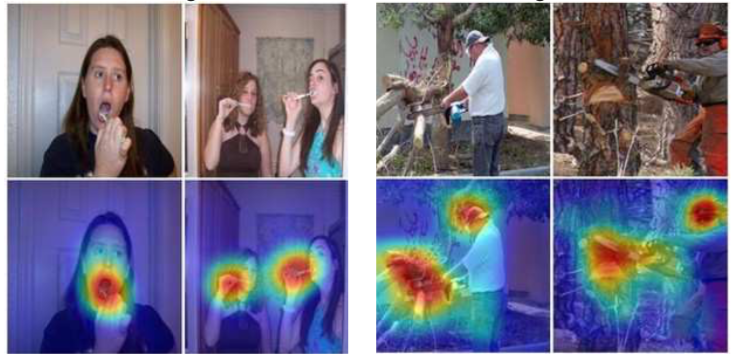
\includegraphics[width=0.5\textwidth]{figure/cam_example.png}
%		\caption{子图1}
%		\label{subfig1}
%	\end{subfigure}
%	\begin{subfigure}{0.45\textwidth}
%		\centering
%		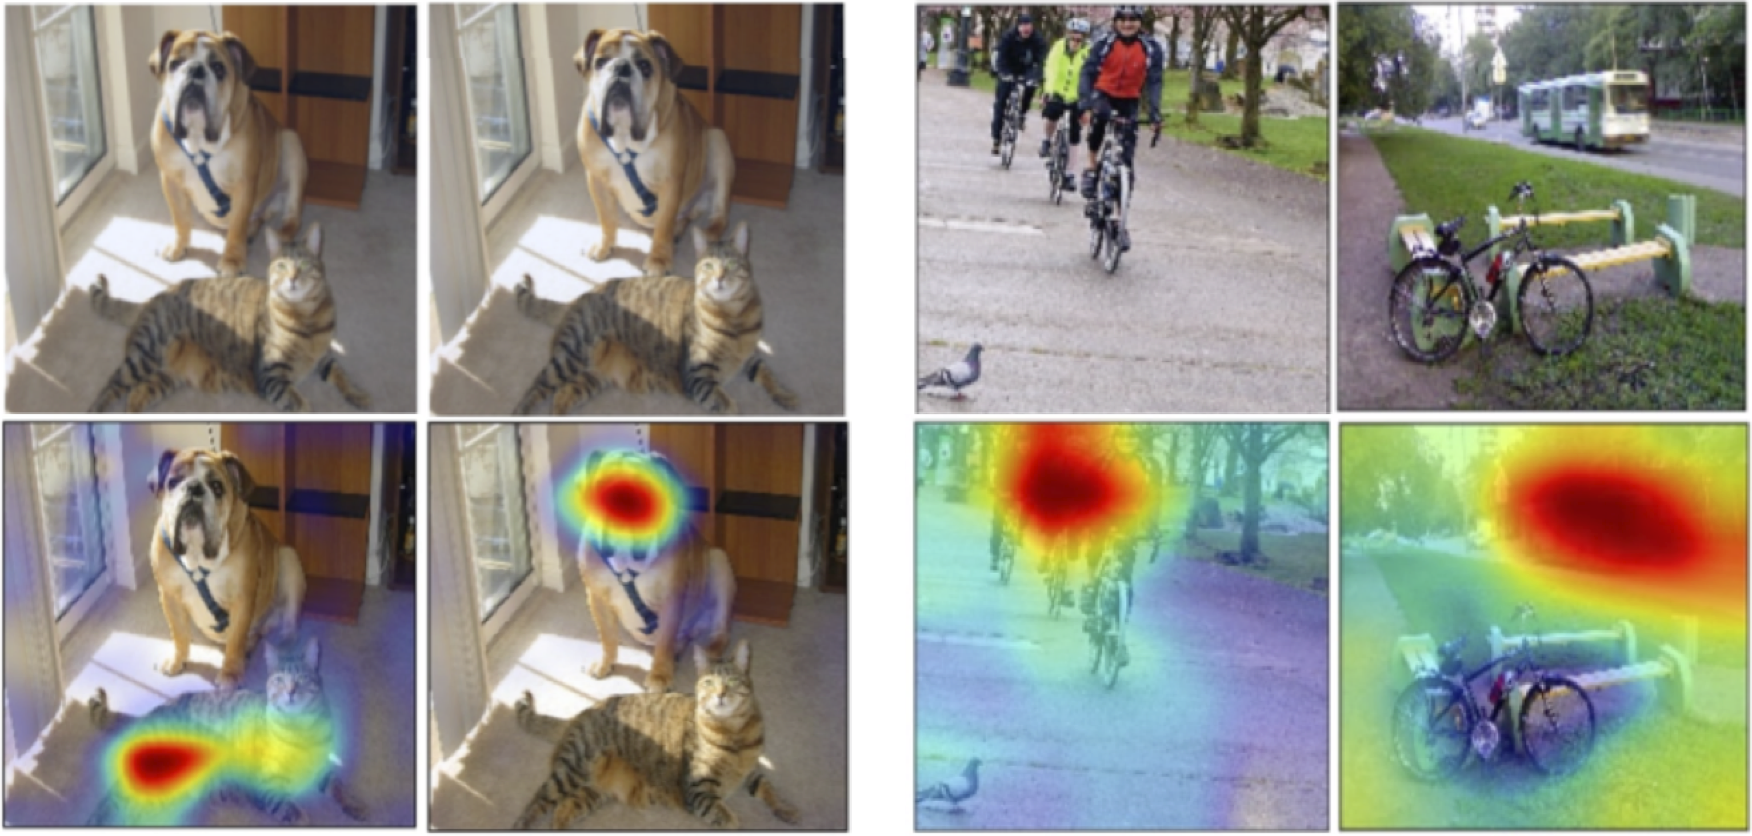
\includegraphics[width=0.5\textwidth]{figure/grad_cam_example.png}
%		\caption{子图2}
%		\label{subfig2}
%	\end{subfigure}
%	\caption{多子图}
%	\label{subfig}
%\end{figure}
\subsubsection*{网络逆转}
网络逆转方法会根据任意层中所有神经元的特征图重建图像,从而揭示该图层中保留了哪些图像信息,也是从网络层角度来解释CNN。网络逆转方法最先用于传统计算机视觉领域,如方向梯度直方图~\cite{dalal2005histograms}(Histogram of Oriented Gradients)。随着CNN的提出与发展,其变体方法~\cite{mahendran2015understanding, mahendran2016visualizing, dosovitskiy2016inverting}开始用于解释CNN。不同的是,Mahendran等人~\cite{mahendran2015understanding, mahendran2016visualizing}使用梯度下降方法从每一层重建图像,而Dosovitskiy等人~\cite{dosovitskiy2016inverting}通过训练专用的向上卷积神经网络(UpconvNet)来重建图像。前者更易于实现,因为它不需要训练额外的专用网络。后者可以通过额外的专用网络可视化更高层的更多现有信息,但是计算成本显著提高。总而言之,这两种算法的主要目标都是从网络层特征图的特定激活中重建原始输入图像。由于基于正则项的网络逆转方法实现相对容易,在此进行更深入的介绍。设给定原始图像$\ve{x}_0$和输入图像$\ve{x}$,基于正则项的网络逆转方法的目标在于重建最优输入图像$\ve{x}^*$,使得损失函数最小,形式化表达为:
\begin{equation}
\ve{x}^{*}=\underset{\ve{x}}{\operatorname{arg\, min}}\left(c \cdot \mathcal{L}\left(\ve{A}(\ve{x}), \ve{A}\left(\ve{x}_{0}\right)\right)+\lambda(\ve{x})\right).
\end{equation}
其中,$\mathcal{L}$是计算输入特定层前后的特征图$\ve{A}(\ve{x}_0)$和$\ve{A}(\ve{x})$的损失函数,$\lambda(\ve{x})$是正则项,$c$是调节损失函数和正则项的超参数。为了让重建图像更像自然图像,$\lambda(\ve{x})$可取L2-范数、全变差范数~\cite{rudin1992nonlinear}等。与激活最大化方法~\cite{simonyan2013deep}相同的是,网络逆转方法也是通过重建输入图像来查看网络层对那些像素或者图像模式更为敏感,但是网络逆转方法可应用到网络任意层,而不限于网络第一层,因而泛化性更强。
%其中,全变差范数可让重建的图像更为平滑。

如果将这些CNN的可视化方法用于定位疾病标记物,可通过可视化图像区域,将CNN分类器在预测图像类别时重点关注的区域看作是疾病标记物。其中,扰动方法~\cite{zintgraf2017visualizing}对每个可能的局部区域进行遮挡或遮罩,并检查分类器输出的变化,输出的下降量越大,说明在预测图像类时的重要性越高。相比之下,特征激活方法则是在特定卷积层输出的特征映射中,根据激活区域来定位重要的局部区域,如流行的类激活映射(CAM~\cite{zhou2016learning})及其变体Grad-CAM~\cite{selvaraju2017grad}等。近年来,基于CAM的方法在医学影像分析中得到了广泛的应用,如胸部X射线图像~\cite{rajpurkar2017chexnet}中肺炎的检测、数字病理图像~\cite{zhang2017mdnet}中膀胱癌的预测、眼底图像中糖尿病性视网膜病变异常区域定位~\cite{Gondaletal17}、胎盘超声影像中胎盘异常定位~\cite{Qi2017WeaklySL}、MRI图像~\cite{yang2018visual}中阿尔茨海默病的诊断等。与CAM和Grad-CAM同样作为一种可视化方法,特征图方法~\cite{simonyan2013deep}利用CNN中的梯度信息计算输入图像中的像素点对图像分类结果的重要性分数。在医学影像处理领域中,该方法可用于解决多通道脑部MRI图像中的肿瘤检测~\cite{banerjee2016novel}、脑部MRI图像中的肿瘤体积检测~\cite{mitra2017volumetric}、皮肤镜图像中的异常分割~\cite{jahanifar2018supervised}等诸多问题。

\subsection{弱监督目标定位}
弱监督目标定位任务是在提供图像级标签的情况下,给出对应类别物体的相关区域。Oquab等人~\cite{Oquab2015IsOL}率先使用CNN描述并解决弱监督目标定位问题,随后一系列运用CNN解决弱监督目标定位问题的方法被提出。在弱监督条件下,解决目标定位任务最常见的思路是利用CNN分类器产生有关于目标位置的监督信号。目标位置的监督信号可以来自于网络本身,还可以由其他方法产生。前者可以理解为一种自监督方法~\cite{2015Hwang},后者可以利用CAM或者Grad-CAM产生目标的位置信息~\cite{Kim_2017_ICCV, Krishna2018}。另外一种思路与CNN可视化中遮挡实验类似,设计多个网络进行对抗性擦除~\cite{WeiFLCZY17, ZhangWF0H18},并采用递归方式生成定位结果,直到分类CNN训练失败。还可以引入注意力机制,让CNN提取的特征更加稀疏,只关注与图像类别相关的区域。

\subsubsection*{生成目标位置的监督信号}
当CNN分类器能够准确地对输入图像分类时,也就能表明CNN分类器已经能够很好学到各个类别图像中具有判别性的特征或者模式,此时便可以利用CNN分类器产生与类别标签相关的目标物体位置信息,从而产生有关目标物体位置的监督信号。Sangheum等人~\cite{2015Hwang}用CNN分类器完成分类任务的同时,用自身CNN分类器产生目标物体的位置信息作为监督信号,借鉴多任务学习思想,同时完成了分类任务和目标定位任务,提出了自迁移学习方法。如图\ref{fig:self_transfer_learning}所示,自迁移学习的损失函数由分类损失和定位损失组成,两者之间设置超参数来平衡权重。在训练的开始阶段,分类网络的损失函数所占权重起着主导作用,因为对于定位器的成功训练,网络权值的初始值是非常重要的,定位器位置信息的监督信号由分类器和定位器共享的CNN特征提取器产生,没有训练良好的特征提取器,就无法产生具有判别性的类别相关区域充当监督信号。随着分类器的性能不断提升,CNN特征提取器产生的监督信号也就越来越可靠,此时需要增加定位损失函数的权重。注意,定位器的监督信号是来自CNN特征提取器本身的,这也是此方法被称作自迁移学习的原因。

\begin{figure}[h]
	\centering
	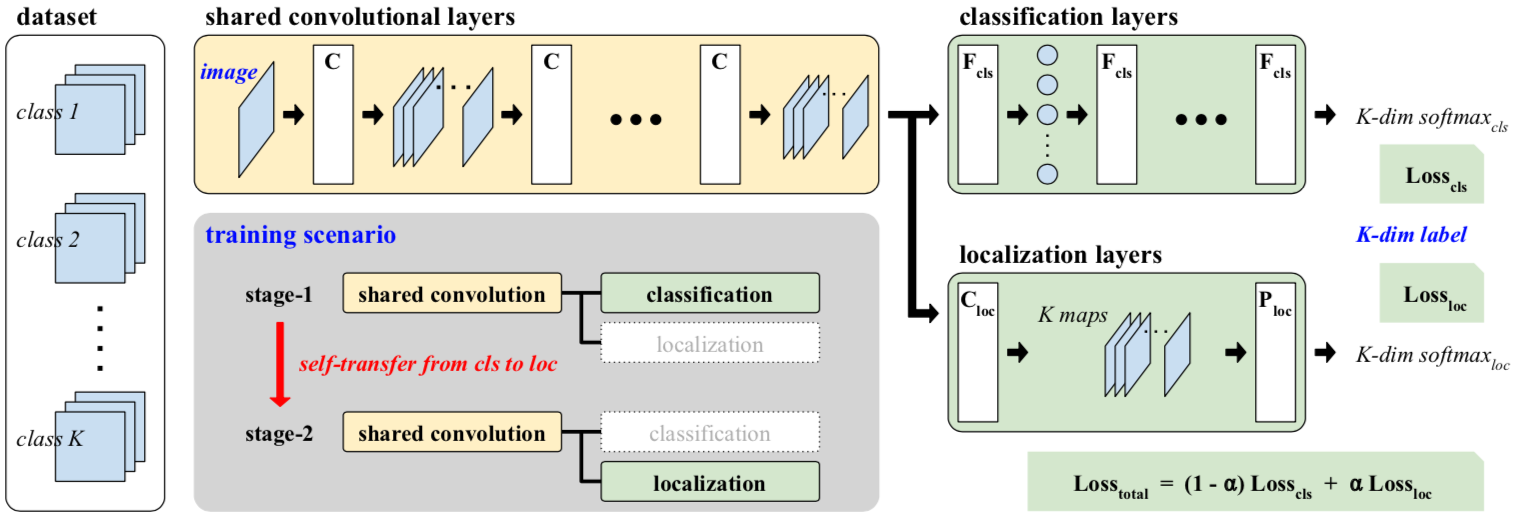
\includegraphics[width=1.0\textwidth]{figure/self_transfer_learning}
	\caption[自迁移学习网络]{自迁移学习网络(图片来自于对应原文~\cite{2015Hwang})。} 
	\label{fig:self_transfer_learning}
\end{figure}
\begin{figure}[h]
	\centering
	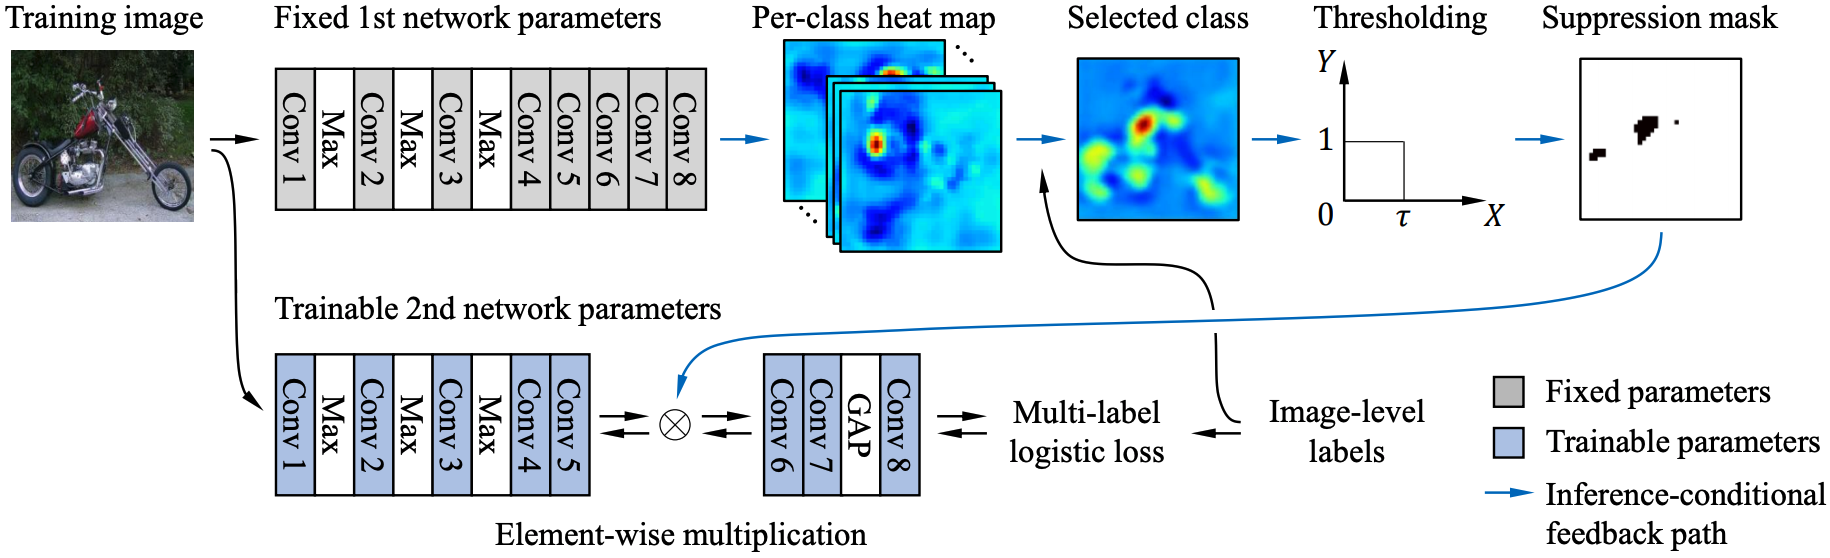
\includegraphics[width=1.0\textwidth]{figure/cam_based_weakly_supervised_localization}
	\caption[利用CAM产生抑制掩码的弱监督目标定位网络]{利用CAM产生抑制掩码的弱监督目标定位网络(图片来自于对应原文~\cite{Krishna2018})。}
	\label{fig:cam_based_weakly_supervised_localization}
\end{figure}

与自迁移学习不同,另外一种思路中位置信息的监督信号来自于其他方法,Kim等人~\cite{Kim_2017_ICCV}提出了一种两阶段训练的方法,第一阶段训练CNN分类器,第二阶段固定第一阶段中的CNN分类器,使用预训练CNN生成的与特定类相关的CAM热图作为抑制掩码,然后将该抑制掩码添加到中间特征图来训练第二个CNN,抑制掩码丢掉了第一阶段中认为的最具有判别性的区域,这会强制第二阶段中CNN分类器去学习除第一阶段外的判别性区域或者模式,最终可通过整合两阶段的结果来更加精确定位到目标物的位置,其网络结构如图\ref{fig:cam_based_weakly_supervised_localization}所示。另外,如果再增加额外训练阶段,可得到更加精细的定位效果。Singh等人~\cite{Krishna2018}同样使用了CAM,与Kim等人等人不同的是,他们通过隐藏输入图像中的部分区域(比如,矩形区域)来迫使网络学习专注于对象的多个相关部分,而不是最相关的部分,还可以将噪声(块)注入到输入图像来进一步加强数据增强,学习到更强大、更鲁邦的目标定位网络。

\subsubsection*{对抗性擦除与注意力机制}
对抗性擦除最初由Wei等人~\cite{WeiFLCZY17}提出,通过对抗性擦除,分类网络首先为特定图像类别标签挖掘最具判别性的区域。然后从图像中删除已发现的判别性区域,并且对分类网络进行了重新训练,以发现一个新的目标区域以尽量保证不会降低分类性能。他们采用递归方式、多次重复这种对抗性擦除过程,直到分类网络训练失败(可将分类网络训练失败定义为对分类网络的可视化结果性能较差或者分类网络分类准确率等评价指标低于某一阈值),再依次将擦除的区域合并为一个完整的前景定位蒙版,其网络模型如图\ref{subfig:adversarial_erasing}所示。由于上述对抗性擦除擦除方法中设置了三个CNN分类器,并且不是端到端训练方式,这需要分多阶段逐步训练CNN,这会造成网络训练时间较长、效率也不够高等缺陷。Zhang等人~\cite{ZhangWF0H18}提出了上述对抗性擦除网络的改进版本,将这些独立的CNN集成到单个网络中,只需要设置两个CNN分类器,并进行端到端的训练,不仅缩短了网络训练周期,还取得了更为优异的定位性能,其网络结构如图\ref{subfig:improved_adversarial_learning}所示。

\begin{figure}[h!]
	\centering
	\begin{subfigure}{0.38\textwidth}
		\centering
		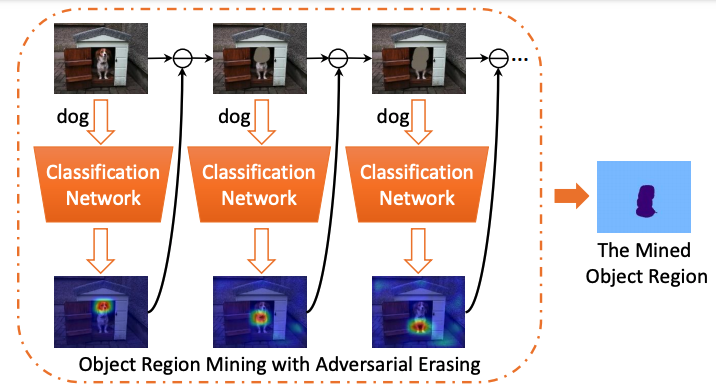
\includegraphics[width=1.0\textwidth]{figure/adversarial_erasing}
        \caption{对抗性擦除网络~\cite{WeiFLCZY17}}
		\label{subfig:adversarial_erasing}
	\end{subfigure}
	%\quad
	\begin{subfigure}{0.57\textwidth}
		\centering
		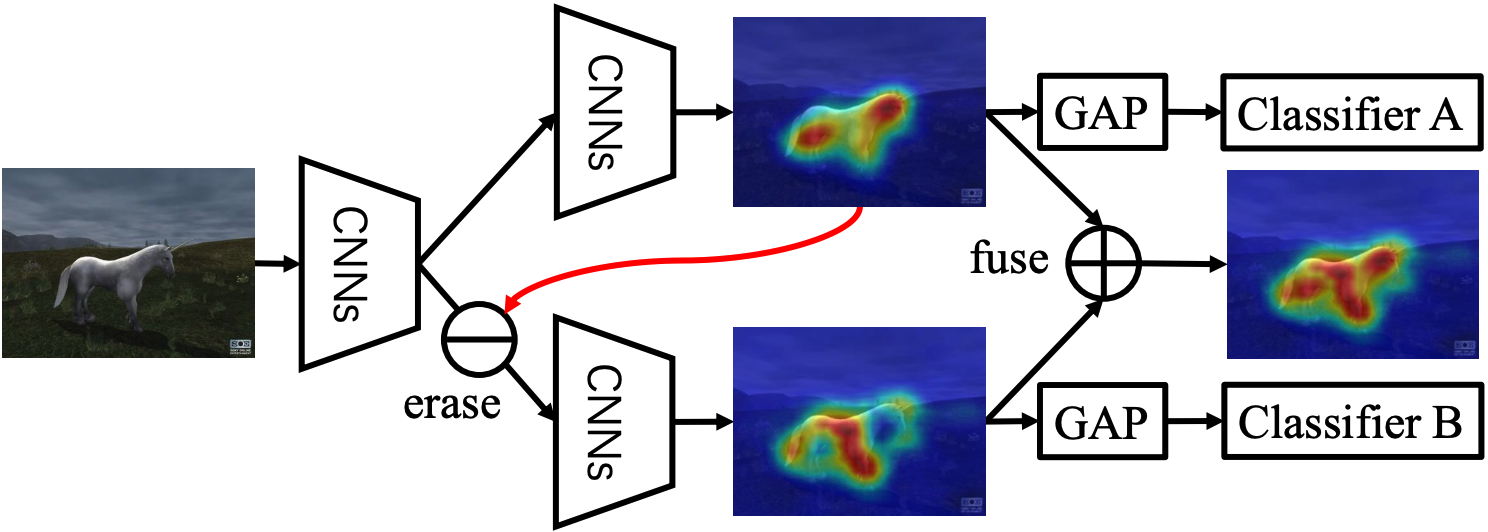
\includegraphics[width=1.0\textwidth]{figure/improved_adversarial_learning}
		\caption{端到端的对抗性擦除网络~\cite{ZhangWF0H18}}
		\label{subfig:improved_adversarial_learning}
	\end{subfigure}
	\caption[两种对抗性擦除网络]{两种对抗性擦除网络(图片均来自于对应原文~\cite{WeiFLCZY17,ZhangWF0H18})。}
	\label{mul_fig:weakly_supervised_localization}
\end{figure}

注意力机制模仿了生物观察行为的内部过程,注意力机制可以快速提取稀疏数据的重要特征,最初被广泛用于自然语言处理任务,特别是机器翻译。在处理计算机视觉问题时,注意力机制可帮助网络关注图像中辅助判断的部分信息,与此同时忽略不相关信息。Teh等人\cite{BMVC2016_52}将注意力机制用于弱监督目标定位,利用注意力机制产生每个特征图的注意力分数,其数值大小表示特征图的重要性程度,从而让分类器能够专注于与特定类最相关的特征或者模式,而目标定位结果可由特征图的加权平均给出,而权值便是对应特征图的注意力分数,其网络结构如图\ref{fig:attention_weakly_supervised_object_localization}所示。
\begin{figure}[h]
	\centering
	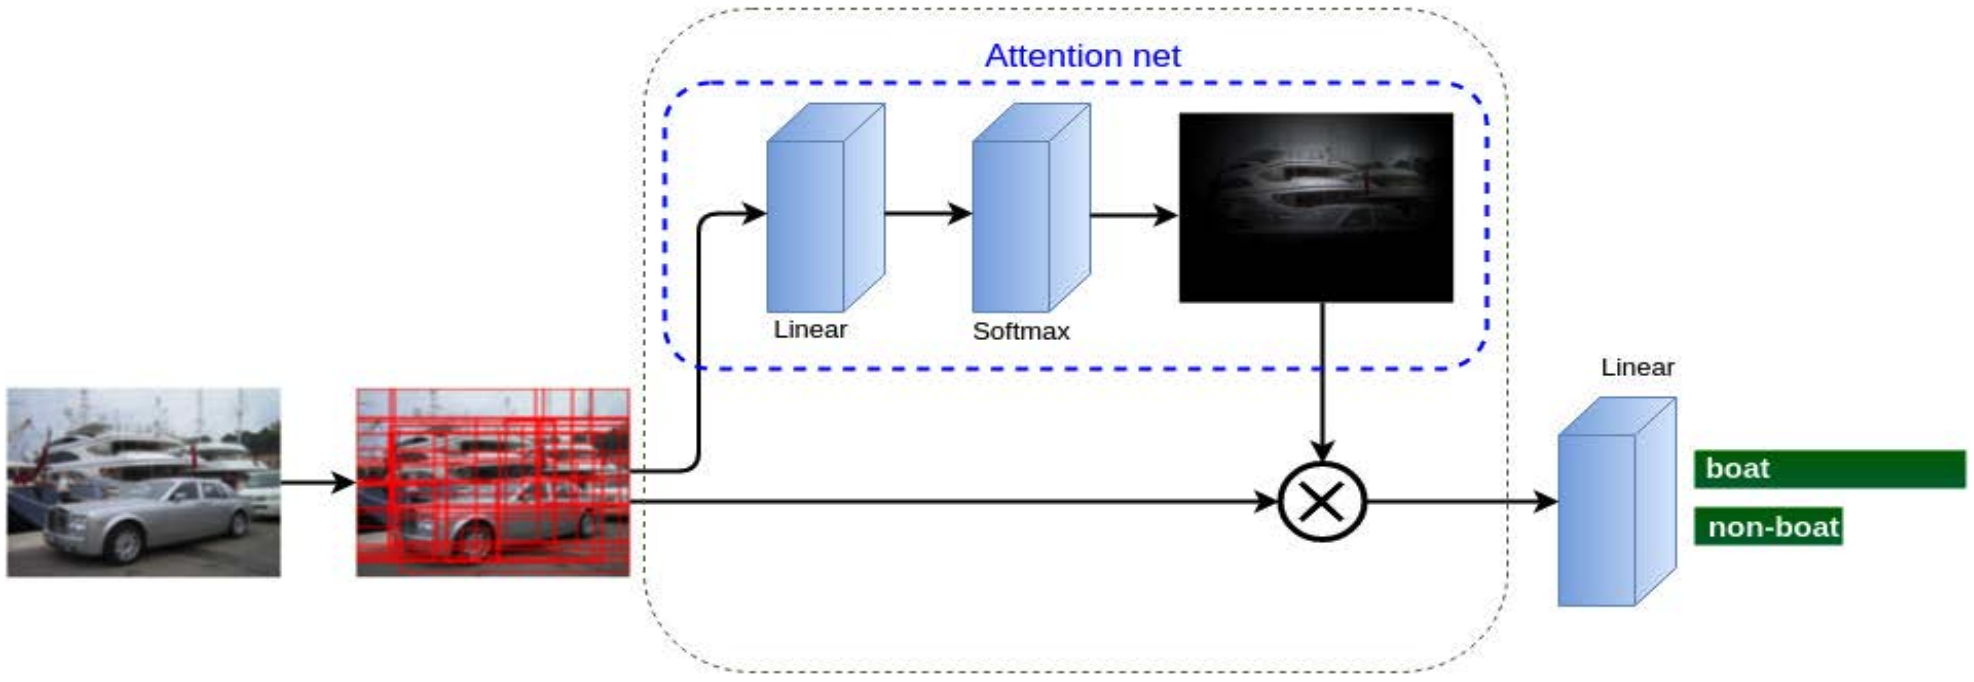
\includegraphics[width=1.0\textwidth]{figure/attention_weakly_supervised_object_localization}
	\caption[引入注意力机制的弱监督目标定位网络]{引入注意力机制的弱监督目标定位网络(图像来自于对应原文~\cite{BMVC2016_52})。}
	\label{fig:attention_weakly_supervised_object_localization}
\end{figure}

近些年来,计算机视觉领域提出的弱监督目标定位方法也被广泛用于定位医学影像中的异常区域。比如,Wang等人~\cite{WangPLLBS17}利用预训练模型产生监督信号辅助定位胸部X射线图像中胸腔疾病病灶,Zhuang等人~\cite{zhuang2019care}利用CAM产生异常区域的监督信号来辅助定位皮肤镜图像中黑色素瘤异常区域和X射线图像中肺炎异常区域。Gonz{\'a}lez-Gonzalo等人~\cite{GonzlezGonzalo2018ImprovingWL}采用循环递归擦除方式不断屏蔽眼底图像中的某些区域来发现判别性区域来定位眼底图像中糖尿病性视网膜病变异常区域,Jim{\'e}nez-S{\'a}nchez等人~\cite{JimnezSnchez2018WeaklySupervisedLA}整合了自迁移学习和CAM定位X射线图像中股骨近端骨折区域,Tang等人~\cite{Tang2018AttentionGuidedCL}直接引入注意力机制来定位X射线图像中胸腔异常区域。Xiao等人~\cite{chen2019cascade}同时添加两个注意力模块来分别关注图像空间信息和通道信息,不仅提高了肝脏异常诊断性能,还较好定位了肝脏病灶区域。

以上内容介绍了与疾病标记物定位任务相关的解决方案,包括MIL、CNN的可视化和弱监督目标定位,其中也不乏优秀精巧的方法,例如CAM和Grad-CAM,但是这些方法的共同劣势在于无法实现像素级的精确定位。一方面,这些方法最初并不是专门为解决疾病标记物定位任务而设计;另一方面,当这些方法被运用到在弱监督条件下疾病标记物定位任务上时,其背后实现原理决定了其无法实现精确的像素级定位,而只能定位到疾病标记物所在的区域或者所聚集的超像素。对于MIL中存在的取块操作,无论其取块尺寸大小,所得图像块都无法避免地包含正常区域。因此MIL方法无法精确定位到疾病标记物。CNN可视化方法中,扰动方法和遮挡方法与MIL一样均需要从图像中取块;激活最大化方法和网络逆转方法只能得到图像的最具判别性的图像特征或者模式;对于基于梯度的方法(比如Grad-CAM),由于在连续卷积作用下特征图通常会不断缩小,因此为了定位到疾病标记物,往往需要将卷积输出响应上采样到输入图像尺寸大小。不难想象,采样倍数越大,疾病标记物的定位越粗糙。如果将疾病标记物也看做是目标物体,那么弱监督目标定位任务的目标是用候选矩形框框出目标物体的位置,该任务目标要求本身就比本文目标低,另外以上弱监督目标定位方法往往需要是通过中间层与目标物体相关的判别性区域来计算目标物体在原图中位置,这个计算过程也会涉及到上采样操作,因而弱监督目标定位方法也无法精确定位疾病标记物。

综上所述,包括MIL、CNN的可视化和弱监督目标定位在内的系列方法都只能粗略定位疾病标记物,精确定位疾病标记物仍是一个有待解决的问题。在弱监督条件下,一种精确定位疾病标记物的新方法亟待提出,这也是本文所有工作的根本出发点。
\section{评价标准}\label{sec:evaluation_metrics}
本文衡量实验结果分为定性分析和定量分析,前者主要比较各种方法得到的定位热图,后者主要把精确率-召回率曲线(Precision-Recall Curve,缩写为P-R Curve)和接收者操作特征曲线(Receiver Operating Characteristic Curve,缩写为ROC Curve)以及对应曲线下的面积(Area Under Curve,缩写为AUC)看作评价标准。
\subsection{接收者操作特征曲线}\label{subsec:roc_curve}
接收者操作特征曲线或者ROC曲线\footnote{https://en.wikipedia.org/wiki/Receiver\_operating\_characteristic}是一个可以说明二元分类器系统的鉴别阈值变化时的诊断能力的图形。通过绘制各种阈值设置下的真阳率(True Positive Rate,缩写为TPR)与假阳率(False Positive Rate,缩写为FPR)来创建ROC曲线。真阳率在机器学习中也称为灵敏度(Sensitivity),表示模型正确预测的正例个数占所有真实正例的比例。假阳率也称为假警报的概率,也可计算为(1-特异性(Specificity)),表示模型预测的假正例(实际为负例)个数占所有真实负例的比例。ROC曲线是以TPR作为衰减的函数。换句话说,ROC曲线的横轴是FPR或者(1-Specificity),纵轴是TPR或者Sensitivity。下面给出TPR、FPR、Sensitivity和Specificity的数学定义。

考虑两类预测问题(二分类),其中标签被标记为正例或负例,以是否是患有糖尿病性视网膜病变为例,我们将患病看作是正例(Positive),将没有患病看作是负例(Negative)。根据分类器给出的预测标签与实际标签是否一致,我们通常有如下定义:

1)真阳(True Positive,缩写为TP):被分类器判定为正例,实际上也是正例。

2)假阳(False Positive,缩写为FP):被分类器判定为正例,但实际上是负例。

3)真阴(True Negative,缩写为TN):被分类器判定为负例,实际上也是负例。

4)假阴(False Negative,缩写为FN):被分类器判定为负例,但实际上是正例。

\noindent 由此,我们可进一步定义TPR、FPR等概念:
\begin{align}
	&\mathrm{TPR}=\mathrm{Sensitivity}=\frac{\mathrm{TP}}{\mathrm{TP}+\mathrm{FN}}\,\, ,\\
	&\mathrm{FPR}=\frac{\mathrm{FP}}{\mathrm{FP}+\mathrm{TN}}\,\, ,\\
	&\mathrm{Specificity}=\frac{\mathrm{TN}}{\mathrm{FP}+\mathrm{TN}}=1-\mathrm{FPR}\,\, .
\end{align}
设在二分类系统中,设$p(0\leq p \leq 1)$表示样本被分为正例的概率。给定$N$个样本,该分类系统给出的预测值为$\ve{x}=\{p_1,p_2,...,p_N
\}$,设这些样本的真实标签为$\ve{y}=\{y_1,y_2,...,y_N\}$,其中$y_i \in \{0,1\},0\leq i \le N$。随后,可依次将二分类系统给出的预测值作为阈值$T(0\leq T \leq 1)$,当$p_i$大于或等于阈值时,我们认为它为正例,否则为负样本。对于多组不同的阈值,我们可以得到多组FPR和TPR,画出ROC曲线。

我们将ROC曲线与横轴正半轴、纵轴正半轴共同围城的面积叫做AUC,AUC数值介于$0.5$与$1$之间,数值大小等于ROC曲线函数沿着FPR在$[0,1]$上的定积分。一般来说,如果一条ROC曲线$f_1$在另外一条ROC曲线$f_2$上方,我们称ROC曲线$f_1$“包围”ROC曲线$f_2$,说明$f_1$代表的分类系统性能优于$f_2$代表的分类系统。
\subsection{精确率-召回率曲线}\label{subsec:pr_curve}
精确率-召回率曲线或者P-R曲线显示了不同阈值时精确率和召回率之间的权衡,是以精确率(Precision)为横轴,召回率(Recall)为纵轴的一条曲线。精确率表示真实正例在被模型识别的正例中的比例,反映了模型识别正例的准确性。召回率也叫检出率,表示被正确识别的正例占所有正例的比例,反映了模型对正例的检索与识别能力。根据\ref{subsec:roc_curve}小节中相关定义,精确率和召回率可定义为:
\begin{align}
	&\mathrm{Precision}=\frac{\mathrm{TP}}{\mathrm{TP}+\mathrm{FP}}\, \, ,\\
	&\mathrm{Recall}=\frac{\mathrm{TP}}{\mathrm{TP}+\mathrm{FN}}\, \, .
\end{align}

P-R曲线是一条以Precision为纵轴,Recall为横轴的曲线。其画法与ROC曲线非常相似,均需要取一组阈值。与ROC曲线的画法不同的是,P-R曲线需要计算Precision和Recall。在ROC曲线中,TPR(纵轴)随着FPR(横轴)的增大而增大,即ROC曲线呈现一种单调增加趋势。而在P-R曲线中,Precision(纵轴)随着Recall(横轴)的增大而减小,即P-R曲线呈现一种单调减小趋势。这种差异主要是Precision和Recall之间的“矛盾”关系造成的。同样,直观上来看,如果一条P-R曲线在另外一条P-R曲线上方,说明前者代表的模型性能优于后者;P-R曲线的AUC定义也与ROC曲线一致,AUC数值越大,模型性能越优。

注意,当测试集中的正负样本的分布变化的时候,ROC曲线能够保持稳定,这是ROC曲线一个重要特征。因此,对于正负样本分布大致均匀的问题,ROC曲线作为性能指标更加鲁邦、更能放映出分类器的优劣。反之,在正负样本分布得极不均匀,负例远大于正例时,P-R曲线对于类别不平衡现象更为敏感、更能反映分类器的性能好坏。
\section{常用数据集}\label{sec:usually_ds_intro}
一旦展开对选取问题的研究工作,第一步便是选取实验所使用的数据集。尤其对于当下十分火热、有着数据驱动特性的深度学习方法来说,选择一个合适的数据集的重要性更加不言而喻。接下来,在已公开的数据集中,本节将简单介绍部分目前在学术界被研究者广泛接受的、图像质量相对较高的数据集。

\subsection{眼底病变数据集}\label{subsec:original_dr_dataset_intro}
眼科学是临床医学的一个独特分支。眼科的影像学检查方法有眼底摄影、光学相干断层扫描、眼底荧光血管造影、扫描激光检眼镜等。在临床实践中,诊断和治疗策略的确定依赖于影像学资料的评价。目前眼底照片已广泛应用于青光眼和视网膜疾病等眼科疾病的诊断。表~\ref{tab:datasets_info}列出了部分眼底病数据集。
\begin{table}[h]
	\centering
	\caption[常用眼底病变数据集]{常用眼底病变数据集。}
	\label{tab:datasets_info}
	\begin{tabular}{c|c|c}
		\toprule[2pt]
		数据集名称 & 图像数量 & 类别 \\
		\midrule[2pt]
		Kaggle Diabetic Retinopathy (DR) Dataset	& $35,127$	& $5$	 \\
		\hline                         
		iChallenge Glaucomatous Optic Neuropathy (GON) Dataset   & $1,200$    & $2$ \\ \hline
		iChallenge Age-related Macular Degeneration (AMD) Dataset & $1,200$    & $2$  \\ \hline
		iChallenge Pathological Myopia (PM)   Dataset            & $1,200$    & $2$ \\ \hline
		Ocular Disease Intelligent Recognition(ODIR)Dataset & $7,000$ & $8$ \\ \hline
		
		Indian Diabetic Retinopathy Image Dataset (IDRiD) & $516$ & $5$  \\
		\bottomrule[2pt]
	\end{tabular}
\end{table}

糖尿病性视网膜病变是目前劳动年龄人口失明的主要原因。DR数据集\footnote{https://www.kaggle.com/c/diabetic-retinopathy-detection/data}是目前关于糖尿病性视网膜病变的最大数据集,提供了在各种成像条件下拍摄的高分辨率视网膜图像。目前在Kaggle上开源数据中,训练集有$35,127$张样本,每张图像尺寸均大于$1000\times 1000$但大小不等,目前只有图像集标注。医生根据患者患病程度将每张图像标注为0至4共5类。标注0、1、2、3和4分别代表未患糖尿病性视网膜病变、轻微糖尿病性视网膜病变、中度糖尿病性视网膜病变、严重糖尿病性视网膜病变和增生性糖尿病性视网膜病变。标注数字越大代表患病程度越严重。

GON数据集\footnote{http://ai.baidu.com/broad/subordinate?dataset=gno}是关于青光眼眼底照片的数据集,共包含$1,200$张彩色眼底照片。并平均分为训练集、验证集和测试集。其中,训练集图像由德国蔡司眼底照相机拍摄,尺寸大小为$2124\times 2056$,验证集和测试集图像由佳能眼底照相机拍摄,尺寸大小均为$1634\times 1634 $。所有图像均是图像级标注,该数据集共有$2$个类别,标记为青光眼/非青光眼,均以后极为中心,伴有黄斑和视盘。

AMD数据集\footnote{http://ai.baidu.com/broad/subordinate?dataset=amd}是关于年龄相关黄斑变性眼底照片数据库,共有$1,200$张彩色眼底照片可供选择。这些照片来自非AMD受试者(约$77$\%)和AMD患者(约$23$\%)。提供AMD/非AMD的标签,椎间盘边界和中央凹的位置,以及各种病变的边界,以训练模型进行自动AMD评估。数据集中每个样本都有图像级标注,只有部分样本有像素级标注,标注了与年龄相关黄斑变性相关的四种典型异常。

近视已成为全球公共卫生的负担。为了促进近视的研究,PM数据集\footnote{http://ai.baidu.com/broad/subordinate?dataset=pm}是病理性近视眼底照片数据库,提供了$1,200$个来自非病理性近视受试者和病理性近视患者(约$50$\%)的视网膜眼底图像。每个图像样本同样均有图像级标注,部分图像有两种典型异常(斑片状视网膜萎缩和视网膜脱离)的像素级标注。

ODIR数据集\footnote{https://odir2019.grand-challenge.org/dataset/}是一个结构化的眼科数据库,其中包括$5,000$名不同年龄的患者的双眼彩色眼底照片和医生的诊断关键词。注意只有来自$3,500$名患者的$7,000$张图像数据作为训练集,并且有图像级标签。该数据集是上工医疗技术有限公司从中国不同医院/医疗中心收集的“真实”患者信息。医生将患者分为$8$个标签,包括正常,糖尿病,青光眼,白内障,年龄相关黄斑变性,高血压,近视和其他疾病/异常。由于存在部分病人同时患有多种疾病,因而部分图像有多个标签。

IDRiD\footnote{https://idrid.grand-challenge.org/Data/}眼底图像是由印度一家眼科诊所的视网膜专家收集的。数据集共包括$516$张样本,均提供了典型糖尿病性视网膜病变和正常视网膜结构的专家标记。数据集所有图像都集中在黄斑附近。图像分辨率为$4288\times 2848$像素,存储为jpg文件格式。此外,它还根据国际临床相关性标准,为数据库中的每张图像提供了关于糖尿病性视网膜病变的疾病严重程度和糖尿病黄斑水肿的信息。与DR数据集一样,它一共将图像分为$5$类。与DR数据集不同的是,IDRiD数据集有$81$张患病彩色眼袋图像有精确像素级标注,比如,微动脉瘤、软渗出物、硬渗出物和出血。

眼底病变图像中通常包含丰富的纹理细节,不同疾病的疾病标记物的视觉特征不尽相同,比如,糖尿病性视网膜病变的疾病标记物广泛分布在视网膜上,疾病标记物的数量众多但单个面积相对较小、不易察觉,而青光眼病变的疾病标记物往往集中分布在视盘附近,疾病标记物的数量很少(多数只有一个)但单个面对相对较大。

\subsection{黑色素瘤皮肤病病变数据集}\label{subsec:original_dermatoscope_ds_intro}
黑色素瘤是多种皮肤癌中最致命的一种。黑色素瘤是发生在皮肤表面的色素性病变,可以通过医生的视觉检查早期发现。黑色素瘤也适用于自动检测与图像分析。皮肤镜检查是一种皮肤成像方法,与无辅助的视觉检查相比,已证明可改善皮肤癌的诊断。在这里,我们介绍三个图像质量较高,可用于疾病标记物定位的黑色素瘤病变皮肤镜数据集。数据集名称、图像数量等基本信息如表~\ref{tab:skin_datasets_info}所示。

\begin{table}[h]
	\centering
	\caption[常用黑色素瘤皮肤病病变数据集]{常用黑色素瘤皮肤病病变数据集。}
	\label{tab:skin_datasets_info}
	\begin{tabular}{c|c|c}
		\toprule[2pt]
		数据集名称 & 图像数量 & 类别 \\
		\midrule[2pt]
		International Skin Imaging Collaboration (ISIC) 2017 Dataset &  $\sim 2,300$ & $3$  \\ \hline
		International Skin Imaging Collaboration (ISIC) 2018 Dataset & $\geq 12,500$ & $7$  \\ \hline
		International Skin Imaging Collaboration (ISIC) 2019 Dataset& $25,331$ & $8$    \\ 
		\bottomrule[2pt]
	\end{tabular}
\end{table}

ISIC2017数据集~\cite{codella2018skin}中大约有$2,300$张皮肤镜图像,其中大约$2,150$张图像是训练集,剩下约$150$张图像是验证集。图像尺寸大小在$400\sim 600$个像素之间。数据集包括黑色素瘤、脂溢性角化病和良性的痣(可看做正常)在内的$3$种类别。

ISIC2018数据集~\cite{codella2019skin, tschandl2018ham10000}中有超过$12,500$张皮肤镜图像。图像尺寸大小在$400\sim 600$个像素之间。包括光化性角化病(日光性角化病)和上皮内癌(鲍文氏病)、基底细胞癌、良性的角化病、皮肤纤维瘤、黑素细胞痣、黑素瘤、血管皮肤损伤共$7$类。

ISIC2019数据集\footnote{https://challenge2019.isic-archive.com/}中有$25,331$张皮肤镜图像,包括黑色素瘤黑素细胞痣、基底细胞癌、光化性角化病、良性角化病(太阳扁豆/脂溢性角化病/扁平苔藓样角化病)、皮肤纤维瘤、血管病变、鳞状细胞癌和没有以上病变类型在内的$8$个类别。图像尺寸大小在$400\sim 600$个像素之间。

与眼底病变类型不同的是,黑色素瘤的各种病变类型往往在皮肤镜上所占区域比较大,通常所占比例在$1/3$以上,另外图像背景以及纹理结构相对简单。

%各种病变类型之间的区别主要表现在病变区域细微纹理区间上。

\section{本章小结}
本章主要先介绍了本文后续内容涉及到的基本知识要点。接着介绍了与疾病标记物定位任务相关的研究进展并阐述了这些方法的劣势。与此同时,也定义了本文实验相关评价标准(ROC曲线及其AUC和P-R曲线及其AUC),最后列举了与疾病标记物定位任务相关的部分数据集。鉴于以上相关工作均无法精确定位疾病标记物这一问题,本文将在第\ref{sec:method}章详细介绍我们提出的解决方法。

%随后,为了验证模型在疾病标记物定位任务上的有效性和鲁棒性,我们在二类问题和多类问题上均进行了相关实验,从P-R曲线和AUC等评价标准上来看,远远超过了CAM和Grad-CAM,验证了我们的模型的先进水平。相关内容我们将会在第\ref{sec:experiments}章进行阐述。